\documentclass{fhnwreport/fhnwreport}

\usepackage{lipsum}
\usepackage[ngerman]{babel}
\usepackage[T1]{fontenc}
\usepackage[utf8x]{inputenc}
\usepackage{tikz}
\usepackage{amsmath}
\usepackage{amsfonts}
%\usepackage{MnSymbol}
\usepackage{wasysym}
\usetikzlibrary{arrows}
\usepackage{lmodern}   %Type1-Schriftart f\"ur nicht-englische Texte
\usepackage{datetime}
\usepackage{cite}
\usepackage{lipsum}
\usepackage{booktabs}
\usepackage{pdflscape}
\usepackage{longtable}
\usepackage{rotating}
\usepackage{xcolor}
\usepackage{colortbl}
\usepackage{hyperref}
\usepackage{appendix}
\usepackage{graphicx}
\usepackage{pdfpages}
\usepackage{enumitem}
\usepackage{caption}
\usepackage{gensymb}
\usepackage{pbox}
\usepackage{draftwatermark}
%\usepackage[nostamp]{draftwatermark}
\usepackage[textsize=footnotesize, textwidth = 17mm, german, colorinlistoftodos]{todonotes}
\usepackage{siunitx}
\usepackage{mathtools}
\usepackage{matlab-prettifier}

\definecolor{dkgreen}{rgb}{0,0.6,0}
\definecolor{gray}{rgb}{0.5,0.5,0.5}
\definecolor{mauve}{rgb}{0.58,0,0.82}

\lstdefinestyle{java}{
    language            = Java,
    aboveskip           = 3mm,
    belowskip           = 3mm,
    showstringspaces    = false,
    columns             = flexible,
    basicstyle          = {\scriptsize\ttfamily},
    numbers             = left,
    numberstyle         = \tiny\color{gray},
    keywordstyle        = \color{blue},
    commentstyle        = \color{dkgreen},
    stringstyle         = \color{mauve},
    breaklines          = true,
    breakatwhitespace   = true,
    tabsize             = 3
}
\lstdefinestyle{Matlab-editor-2}{%
  style               = MatlabBaseStyle@mlpr,
  mllastelementstyle  = \color{black}                    ,
  mlkeywordstyle      = \color[RGB]{000,000,255}         ,
  mlcommentstyle      = \color[RGB]{034,139,034}         ,
  mlstringstyle       = \color[RGB]{160,032,240}         ,
  mlsyscomstyle       = \color[RGB]{178,140,000}         ,
  mlsectiontitlestyle = \commentStyle@mlpr      \bfseries,
  mlsharedvarstyle    = \color[RGB]{000,163,163}         ,
  mlplaceholderstyle  = \mleditorphstyle,
  basicstyle          = \ttfamily\scriptsize,
  numbers             = left,
}


\SetWatermarkText{\texttt{Entwurf}}
\SetWatermarkText{Entwurf}
\SetWatermarkLightness{0.9}

\setcounter{secnumdepth}{5}
\setcounter{tocdepth}{2}

\DeclarePairedDelimiter\abs{\lvert}{\rvert}%

\renewcommand{\thesubsubsection}{\arabic{subsubsection}}

\hypersetup{%
  bookmarksnumbered = true,
  colorlinks = true,
  linkcolor  = black,
  citecolor  = black,
  %urlcolor   = blue,
  urlcolor   = black,
  %hidelinks  = false
}

\title{%
    \vspace{40mm}
    \Huge{Reglerdimensionierung mittels Phasengangmethode} \\
    \vspace{20mm}
    \huge{Fachbericht}
    \date{\today}
}

\newcommand{\colfigure}[3]{%
    \begin{minipage}[c][][b]{0.485\textwidth}
        #1
    \end{minipage}
    \hspace{0.03\textwidth}
    \begin{minipage}[c][][b]{0.485\textwidth}
        {\raggedleft%
            \includegraphics[width=0.9\textwidth]{#2}%
        }
        \captionof{figure}{#3}
    \end{minipage}\\%
}

\newlist{longenum}{enumerate}{5}
\setlist[longenum,1]{label=\roman*)}
\setlist[longenum,2]{label=\alph*)}
\setlist[longenum,3]{label=\arabic*)}
\setlist[longenum,4]{label=(\roman*)}
\setlist[longenum,5]{label=(\alph*)}

\def\code#1{\texttt{#1}}



\usepackage{pdfpages}

\begin{document}

\begin{titlepage}

    \maketitle

    \vspace{20mm}

    %\hspace{-20mm}
    \begin{tabular}{r|l}

        \textsc{\textbf{Studiengang}}
        & EIT\\
        [4mm]

        \textsc{\textbf{Modul}}
        & Projekt 2 \\
        [4mm]

        \textsc{\textbf{Team}}
        & 4 \\
        [4mm]

        \textsc{\textbf{Auftraggeber}}
        & Peter Niklaus \\
        [4mm]

        \textsc{\textbf{Fachcoaches}}
        & Peter Niklaus, Richard Gut, Pascal Buchschacher, Anita Gertiser \\
        [4mm]

        \textsc{\textbf{Autoren}}
        & Anita Rosenberger, Benjamin M\"uller, Manuel Suter, Florian Alber, Raphael Frey\\
        [4mm]

        \textsc{\textbf{Version}}
        & \code{1} \\
    \end{tabular}
    %\end{center}

\end{titlepage}



% **************************************************************************** %
\thispagestyle{empty}
\section*{Abstract}
\label{sec:abstract}
% **************************************************************************** %
% Problemstellung (Welches Problem wurde gelöst? Welche Aufgabe war zu erfüllen? In welchem Gebiet wurde es gelöst?)
Im Gebiet der Regelungstechnik ist das Dimensionieren von Regler eine zentrale Aufgabe, da mit der korrekten Einstellung der Regler stabil und die Differenz zwischen Ist und Soll-Wert möglichst klein ist.\\
Die Phasengangmethode ist eine ursprünglich eine graphische Berechnungsart, welche anhand der Schrittantwort die Reglerwerte berechnet. Die Aufgabe der Implementierung dieser Methode in Java war die Hauptaufgabe.\\
\\
%Ziel/Anforderungen (Was soll unter welchen Bedingungen/Berücksichtigungen erreicht werden?)
Die Ziel dieses Projektes war, ein  benutzerfreundliches Softwaretool, das heisst auch für ein ungeübter Regelungstechniker benutzen kann,  zu entwickeln, welches anhand der Phasengangmethode die Dimensionierung eines PI und PID Reglers durchführt. Die Ausgabe des   Tools soll anhand der Eingabe der Schrittantwortwerte die numerische wie auch die graphische Lösung ausgeben.\\
\\
%Methodik: (Wie wurde das Problem angegangen?)
Die Phasengangmethode und die als Vergleich angewendete Faustformeln wurden in Matlab geschrieben und mit Referenzdaten getestet. Die Implementierung in Java war ein zweistufiger Prozess, in welchem zuerst die matlabtypischen Berechungsfunktionen ausprogrammiert  und im zweiten Schritt die Regeldimensionierung implementiert wurden.\\
\\
%Hauptresultate
Das Softwaretool besitzt eine graphische Benutzeroberfläche, über welche auf der linken Seite die Werte der Schrittantwort eingelesen und die numerserischen Lösungen des Reglers ausgegeben  und über die rechte Seite die graphischen Lösungen dargestellt werden.\\
\\
%Konklusion (Schlussfolgerung; Was ist das Zentrale an der Lösung? Was ist das Neue an der Lösung?
Das Zentrale an der Lösung ist die Berechungungseschwindigkeit mit welcher das Tool arbeitet. Dies ermöglicht eine "Echtzeit" Dimensionierung des Reglers. Das Neue an dieser Lösung ist das Einbinden der Phasengangmethode in ein Reglerdimensionierungstool.


% **************************************************************************** %
\clearpage
\thispagestyle{empty}
% \section*{Aufgabenstellung}
% \label{sec:aufgabenstellung}
% **************************************************************************** %



%
\includepdf[pages=-,scale=1]{images/AufgabevomAuftraggeber}
%
\includepdf[pages=-]{images/AufgabevomAuftraggeber.pdf} 



% **************************************************************************** %
\pagestyle{empty}
{
    \renewcommand{\thispagestyle}[1]{}
    \tableofcontents
    \vspace{80mm}
    \subsection*{Versionsgeschichte}
    \begin{itemize}
        \item[]
            \emph{10.06.2015:} \texttt{Version 1}
    \end{itemize}
}

\clearpage
\setcounter{page}{1}
\pagestyle{headings}
% **************************************************************************** %



% **************************************************************************** %
\clearpage
\section{Einleitung}
\label{sec:einleitung}
% **************************************************************************** %
Im Rahmen dieses Projektes soll ein  Tool entwickelt werden, welches einen PI-  % Ausgangslage
respektive einen PID-Regler mittels der von Prof. Jakob Zellweger entwickelten
Phasengangmethode  \todo{referenz script Zellweger}                                                             
dimensioniert. Zum Vergleich  soll der entsprechende Regler  ebenfalls mittels
verschiedenen  Faustformeln ausgelegt  werden. Die  Phasengangmethode ist  ein
graphisches Werkzeug,  das normalerweise  mit Stift und  Papier durchgef\"uhrt
wird. Folglicherweise  ist seine  Ausf\"uhrung zeitaufw\"andig,  speziell wenn
verschiedene  Szenarien  mit unterschiedlichen  Parameterwerten  durchgespielt
werden sollen. Ein Tool zur Automatisierung  dieses Prozesses ist bisher nicht
verf\"ugbar; unsere Software soll diese Marktl\"ucke f\"ullen.

Das Tool soll ausgehend von drei Parametern aus der Schrittantwort der Strecke  % Anforderungen
(Verst\"arkung  $K_s$, Anstiegszeit  $T_g$, Verz\"ogerungszeit  $T_u$) mittels
der Phasengangmethode  m\"oglichst ideale  Regelparameter berechnen  sowie die
Schrittantwort  des darauf  basierenden  geschlossenen Regelkreises  graphisch
darstellen. Die Benutzeroberfl\"ache  der Software soll intuitiv  sein, sodass
sich auch mit  dem Thema nicht eingehend  vertraute Regelungstechniker einfach
zurechtfinden.

Die  erforderlichen   Algorithmen  wurden  eigenst\"andig  zuerst   in  Matlab % Umsetzung.  
als  Prototypen   implementiert  und   anschliessend  vollst\"andig   in  Java\todo{mehr/anderer Inhalt?}
konvertiert. Auch die  graphische Benutzeroberfl\"ache baut ganz  auf Java. Um
optimale  Wartbarkeit,  \"Ubersichtlichkeit  und Modularit\"at  des  Codes  zu
gew\"ahrleisten,  ist  die  Software  gem\"ass  Model-View-Controllern-Pattern
aufgebaut.

Nach  der Berechung  in  Matlab  wurde klar,  dass  die  Berechnung durch  die % Ergebnisse
hohe Rechenleistung  sehr schnell  durchgef\"uhrt werden  kann und  somit eine
Dimensionierung des geschlossenen Regelkreises anhand dieser Methode von Herrn
Zellweger m\"oglich ist.

Das  Projekt gliederte  sich prim\"ar  in  zwei Teile. In  einer ersten  Phase % Aufbau des Berichts.
wurden  die  theoretischen  Grundlagen erarbeitet,  darauf  aufbauend  bestand
die  zweite  Phase  vor  allem   aus  der  Implementierung  der  Software. Der
vorliegende Bericht entspricht in seinem  Aufbau diesem Verlauf und beschreibt
die erarbeitete Theorie und die entwickelte Software.



% **************************************************************************** %
\clearpage
\section{Grundlagen der Regelungstechnik}
\label{sec:grundlagenRegtech}
% **************************************************************************** %
% ---------------------------------------------------------------------------- %
\subsection{Die Steuerung}
% ---------------------------------------------------------------------------- %

Unter einer Steuerung  versteht man eine offen Wirkungskette  wie in Abbildung
\ref{fig:Steuerung},   dass  heisst   die  Wirkglieder   sind  ketten\"ahnlich
aufgereiht und besitzen keine R\"uckkopplung. Die Steuerkette wird genau f\"ur
eine Steuerung ausgelegt und kann  nur auf Steuergr\"ossen reagieren. Ohne die
R\"uckkopplung wird das Ausgangsignal  nicht mit dem Eingangssignal verglichen
und es k\"onnen keine Korrekturen vorgenommen werden.

\begin{figure}[!h!, width=\pagewidth]
    \centering
    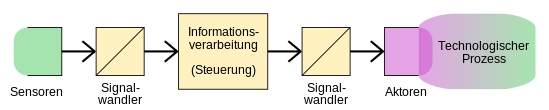
\includegraphics[width=0.5\textwidth]{images/Steuerung}
    \caption{Steuerung}
    \label{fig:Steuerung}
\end{figure}


% ---------------------------------------------------------------------------- %
\subsection{Der geschlossene Regelkreis}
\label{subs:grundl:geschlossenerRegelkreis}
% ---------------------------------------------------------------------------- %
Die      Aufgabe     eines      geschlossenen     Regelkreises      (Abbildung
\ref{fig:geschlossenerRegelkreis})  ist  es,   einen  vorgegeben  Sollwert  zu
erreichen und diesen  auch bei St\"orungen aufrecht  zu erhalten. Dabei sollen
die unten  genannten dynamischen  Anforderungen eingehalten werden,  damit die
Stabilit\"at des Regelsystems garantiert ist. Daraus folgt auch die wichtigste
Bedienung f\"ur  die Schrittantwort ein geschlossenen  Regelkreis heisst, dass
der Regelfehler, die Differenz zwischen Ist- und Sollwert, m\"oglichst schnell
gleich Null oder m\"oglichst klein ist.


\begin{figure}[!h!, width=\pagewidth]
    \centering
    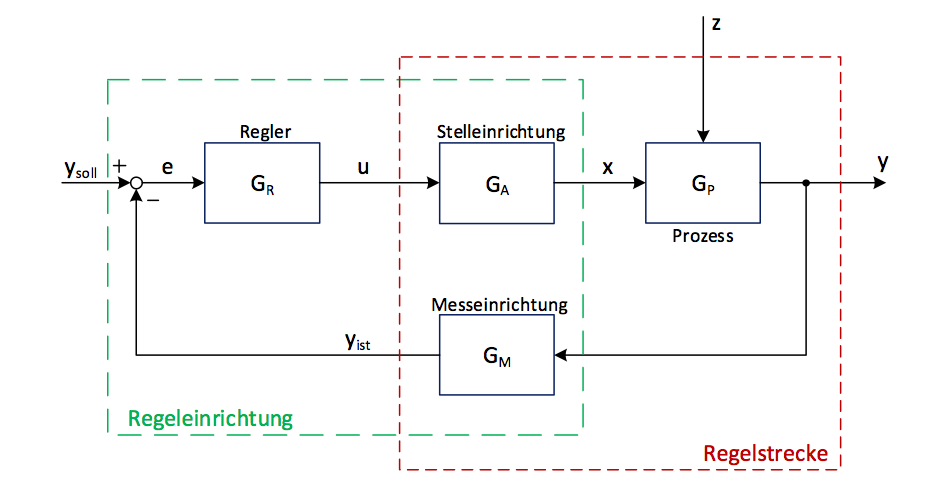
\includegraphics[width=0.5\textwidth]{images/geschlRegelkreis}
    \caption{Geschlossener Regelkreis}
    \label{fig:geschlossenerRegelkreis}
\end{figure}

%Name Bild Struktur eines allgemeinen Regelkreises
\begin{itemize}
    \item
        $y_{soll}$ bezeichnet den Sollwert der Regelgr\"osse
    \item
        $e$ Regelabweichung (Regelfehler)
    \item
        $u$ Steuergr\"osse
    \item
        $x$ Stellgr\"osse
    \item
        $y$ Regelgr\"osse
    \item
        $z$ St\"orgr\"ossen werden in diesem Projekt nicht ber\"ucksichtigt
    \item
        $y_{ist}$ ist  der Ist-Wert  der Regelgr\"osse und  wird auch  als die
        Schrittantwort des Regelkreises bezeichnet.
\end{itemize}


Grunds\"atzlich  k\"onnen  f\"unf   Anforderungen  f\"ur  einen  geschlossenen
Regelkreis und seinen Schrittantworten zusammengefasst werden:
\begin{enumerate}
    \item
        Der Regelkreis muss stabil  sein: F\"ur das Regelsystem heisst stabil,
        dass es in seinen Gleichgewichtszustand zur\"uckgef\"uhrt werden kann.
    \item
        Der Regelkreis muss gen\"ugend ged\"ampft sein.
    \item
        Der   Regelkreis   muss   eine  bestimmte   station\"are   Genauigkeit
        aufweisen: Das   bedeutet,    der   Regelfehler   e(t)    soll   f\"ur
        $t\rightarrow\infty$ gegen null gehen.
    \item
        Der  Regelkreis  muss  hinreichend schnell  sein: Ist  die  D\"ampfung
        zu  stark   oder  zu  schwach,  braucht   der  Einschwingvorgang  mehr
        Zeit. Hierbei  muss  darauf  geachtet werden,  dass  die  spezifischen
        Anforderungen an das Regelsystem eingehalten werden.
    \item
        Der  Regelkreis muss  robust  sein: Der Regelkreis  muss so  ausgelegt
        werden,  dass  das  Regelsystem  auch im  schlimmsten  Fall  (je  nach
        Regelsystem situationsabh\"angig) in der Lage ist, das System zur\"uck
        in den stabilen Zustand (vgl. 1.) zu regeln.
\end{enumerate}


% ---------------------------------------------------------------------------- %
\subsubsection*{Die Schrittantwort des geschlossenen Regelkreises}
% ---------------------------------------------------------------------------- %

\begin{figure}[h!, width=\pagewidth]
    \begin{center}
    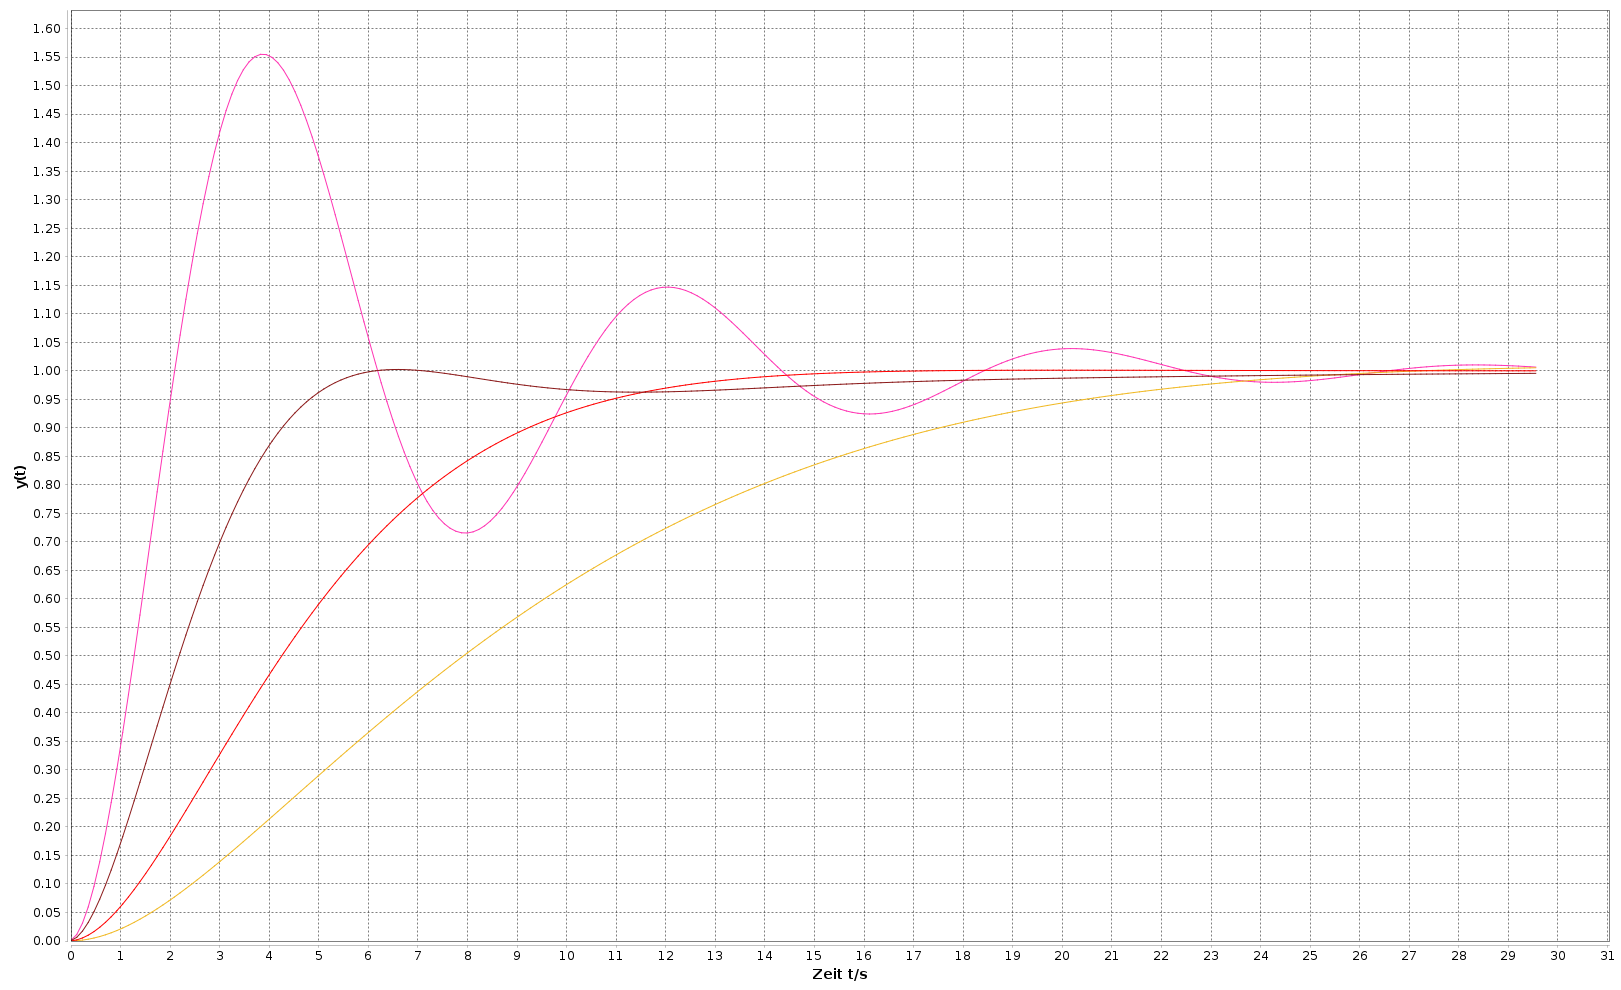
\includegraphics[width=0.8\textwidth]{images/schrittantworten.png}
    \caption{Schrittantworten verschiedener Charakteristiken}
    \label{fig:stepresponse}
    \end{center}
\end{figure}

Als Schrittantwort eines geschlossenen Regelkreises wird der zeitliche Verlauf
des Ausgangssignals  $y(t)$ bezeichnet,  welches entsteht wenn  $y_{soll}$ von
$0$  auf  $1$ springt. In  der  Abbildung  \ref{fig:stepresponse} werden  drei
verschiedene Schrittantworten gezeigt.  Im  Zusammenhang mit den Anforderungen
an  den  geschlossenen  Regelkreis,  werden  an  die  Schrittantwort  folgende
Forderungen gestellt:

\begin{enumerate}
    \item
        Die Schrittantwort eines stabilen Regelkreises darf nach dem Erreichen
        des eingeschwungenen Zustands kein erneutes \"Uberschwingen auftreten.
    \item
        Die  D\"ampfung  der  Schrittantwort  soll so  stark  sein,  dass  der
        eingeschwungene Zustand m\"oglichst rasch erreicht wird ohne, dass das
        \"Uberschwingen des Systems zu stark  wird. Die dunkel orange Kurve in
        Abbildung \ref{fig:stepresponse} zeigt eine Schrittantwort, welche vor
        dem Erreichen des eingeschwungenen Zustands, \"uberschwingt.
    \item
        Die   Schrittantwort  muss   f\"ur  ein   $t\rightarrow\infty$  gleich
        $y_{soll}$ sein.
    \item
        Die Schnelligkeit des Einschwingvorganges der Schrittantwort ist stark
        von der  D\"ampfung abh\"angig. Wenn  diese zu  stark oder  zu schwach
        ist, ist der Regelkreis zu langsam. Die hell orange Kurve in Abbildung
        \ref{fig:stepresponse} zeigt eine zu langsame Schrittantwort.
\end{enumerate}

Die  Berechnung   der  Schrittantwort  des  geschlossenen   Regelkreises  wird
in  unserem   Tool  mittels  der  inversen   schnellen  Fourier-Transformation
durchgef\"uhrt, genauere  Informationen dazu sind  in Abschnitt~\ref{subs:fft}
und Anhang~\ref{app:algo:ifft} zu finden.


% ---------------------------------------------------------------------------- %
\subsection{Regelstrecke}
% ---------------------------------------------------------------------------- %

In  der  Regelungstechnik  wird  die  zu  regelnde  Strecke  als  Regelstrecke
bezeichnet. Die  zu   regelnde  Strecke   ist  zum  Beispiel   die  Temperatur
im  Raum  oder  die  Luftfeuchtigkeit  in  der  Sauna. Die  Regelstrecke  wird
durch  ihr   Zeitverhalten  charakterisiert,  welches  den   Aufwand  und  die
G\"ute   der   Regelung   bestimmt. Um  das   Zeitverhalten   zu   beschreiben
verwendet  man die  Sprungantwort,  welche zeigt,  wie  die Regelgr\"osse  auf
Stellgr\"ossen\"anderung reagiert. Mit  der entstehenden  Regelgr\"osse werden
verschiedene Regelstrecken unterschieden:

\begin{itemize}
    \item
        P-Regelstrecke
    \item
        I-Regelstrecke
    \item
        Strecken mit einer Totzeit
    \item
        Strecken mit Energiespeicher
\end{itemize}

Dieses  Projekt   besch\"aftigt  sich   mit  den  PTn-Strecken,   welche  eine
Kombination  aus einer  Strecke  mit proportionalen  Verhalten  und einer  mit
Totzeit ist. Die Ordnung der Strecke ist in n angegeben.

\subsubsection*{P-Regelstrecke}
Bei  der  Regelstrecke mit  proportionalem  Verhalten  folgt die  Regelstrecke
proportional der  Stellgr\"osse ohne  Verz\"ogerung. Dies kommt in  der Praxis
nicht vor,  da immer eine  Verz\"ogerung vorhanden ist. Ist  die Verz\"ogerung
jedoch  sehr  klein  spricht  man   von  einer  P-Strecke. Das  Verhalten  der
Strecke  ist in  ihrem Blockschaltbild  (Abb. \ref  {fig:PStrecke}) symbolisch
dargestellt. Der  Proportionalit\"atsfaktor wird  mit $K_p$  abgek\"urzt. Wird
$K_p<1$ wirkt $K_p$ nicht mehr verst\"arkend sondern abschw\"achend.

\begin{figure}[h!, width=\pagewidth]
    \centering
    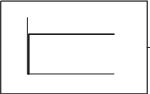
\includegraphics[width=0.2\textwidth]{images/PStrecke}
    \caption{Blockschaltbild von P-Strecke}
    \label{fig:PStrecke}
\end{figure}


% ---------------------------------------------------------------------------- %
\subsubsection*{Strecken mit Totzeit}
% ---------------------------------------------------------------------------- %

\"Andert  sich  die  Stellgr\"osse,  wirkt sich  diese  \"Anderung  bei  einer
Strecke  mit Totzeit  erst  nach  einer gewissen  Zeit  auf die  Regelgr\"osse
aus. Mit $T_t$  wird das  Mass der Totzeit  gekennzeichnet. Im Blockschaltbild
(Abb.  \ref{fig:TotZeit}) wird  die  Totzeit durch  ein  Unterbruch am  Anfang
gekennzeichnet.

Totzeiten     verursachen    schnelle     Schwingungen,     da    sich     die
Stellgr\"osse\"nanderung zeitverz\"ogert  auf die  Regelgr\"osse auswirkt. Die
Schwingungen  entstehen  wenn sich  die  Stellgr\"osse  und die  Regelgr\"osse
periodisch \"andern.

\begin{figure}[h!, width=\pagewidth]
    \centering
    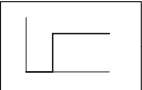
\includegraphics[width=0.2\textwidth]{images/TotZeit}
    \caption{Blockschaltbild von Strecke mit Totzeit}
    \label{fig:TotZeit}
\end{figure}


% ---------------------------------------------------------------------------- %
\subsubsection*{I-Regelstrecke}
% ---------------------------------------------------------------------------- %

Die  I-Regelstrecke  antwortet  auf eine  Stellgr\"ossen\"anderung  mit  einer
fortw\"ahrenden \"Anderung in steigende oder fallende Richtung. Die Begrenzung
dieses   Vorganges  ist   mit  den   systembedingten  Schranken   gegeben. Die
Integrierzeit  $T_i$  ist  ein  Mass  f\"ur  die  Anstiegsgeschwindigkeit  der
Regelgr\"osse  und das  Blockschaltbild  (Abb.  \ref{fig:IStrecke}) zeigt  das
Verhalten sinnbildlich.

\begin{figure}[h!, width=\pagewidth]
    \centering
    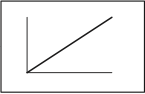
\includegraphics[width=0.2\textwidth]{images/IStrecke}
    \caption{Blockschaltbild von I-Strecke}
    \label{fig:IStrecke}
\end{figure}


% ---------------------------------------------------------------------------- %
\subsection{Regler}
% ---------------------------------------------------------------------------- %

Die Aufgabe  eines Reglers  besteht darin  die zu  regelnde Strecke  mit einem
Stellsignal  so  zu  beeinflussen,  dass der  Wert  der  Regelgr\"osse  gleich
dem  Wert  der F\"uhrungsgr\"osse  entspricht. Der  Regler  besteht aus  einem
Vergleichsglied,  welches  die  Reglerdifferenz  aus  der  Differenz  zwischen
F\"uhrungs-  und Reglergr\"osse  bildet und  dem Reglerglied. Das  Reglerglied
erzeugt aus der Reglerdifferenz die Stellgr\"osse.

Es wird zwischen P-, I- und D-Regler unterschieden.

In diesem Projekt werden die PI- und PID-Regler, welche Kombinationen der oben
genannten Regler sind, behandelt.


% ---------------------------------------------------------------------------- %
\subsubsection{PI-Regler}
% ---------------------------------------------------------------------------- %
Der  PI-Regler   besteht  aus  einer   Parallelschaltung  von  einem   P-  und
einem  I-Regler (Abb.\ref{fig:PIRegler}). Durch  diese Kombination  werden die
Nachteile  beider  Regler  aufgehoben   und  die  Vorteile  (schnell,  stabil)
hervorgehoben. Sein  Verhalten   wird  bildlich  in  dem   Blockschaltbild  in
Abbildung \ref{fig:PIRegler2} dargestellt.

\begin{figure}[h!, width=\pagewidth]
    \centering
    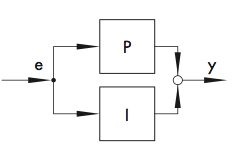
\includegraphics[width=0.4\textwidth]{images/PIRegler1}
    \caption{Parallelschlatung von P-Regler und I-Regler}
    \label{fig:PIRegler1}
\end{figure}

\begin{figure}[h!, width=\pagewidth]
    \centering
    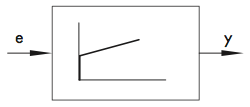
\includegraphics[width=0.4\textwidth]{images/PIRegler2}
    \caption{Blockschaltbild von PI-Regler}
    \label{fig:PIRegler2}
\end{figure}


% ---------------------------------------------------------------------------- %
\subsubsection{PID-Regler}
% ---------------------------------------------------------------------------- %

Wird    dem    PI-Regler    ein    D-Anteil    parallel    geschaltet    (Abb.
\ref{fig:PRDRegler1}), entsteht  der PID-Regler. Der  PID-Regler ist  ein sehr
oft verwendeter  Regler, da durch  den D-Anteil die Regelgr\"osse  rascher den
Sollwert erreicht  und der Einschwingvorgang schneller  abgeschlossen ist. Das
Blockschaltbild  zeigt dieses  Verhalten (Abb.\ref{fig:PID})  anschaulich. Der
PID-Regler  ist   geeignet  f\"ur  Regelstrecken  h\"oherer   Ordnung,  welche
m\"oglichst  schnell  und  ohne bleibende  Regelabweichungen  geregelt  werden
m\"ussen.

\begin{figure}[h!, width=\pagewidth]
    \centering
    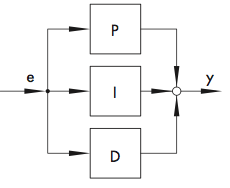
\includegraphics[width=0.4\textwidth]{images/PRDRegler1}
    \caption{Parallelschaltung von P-, I-, und D-Regler}
    \label{fig:PRDRegler1}
\end{figure}

\begin{figure}[h!, width=\pagewidth]
    \centering
    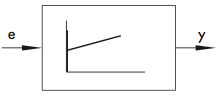
\includegraphics[width=0.4\textwidth]{images/PIDRegler2.png}
    \caption{Blockschaltbild des PID-Reglers}
    \label{fig:PID}
\end{figure}



% **************************************************************************** %
\clearpage
\section{Fachlicher Hintergrund zur Reglerdimensionierung}
\label{sec:fachlicher_hintergrund}
% **************************************************************************** %
Das  Kernst\"uck  dieser Arbeit  und  des  zugeh\"origen Softwaretools  stellt
die   sogenannte   \emph{Phasengangmethode  zur   Reglerdimensionierung}   von
Jakob   Zellweger   dar~\cite{regelungstechnik:zellweger_short}. Diese   wurde
urspr\"unglich  als  vereinfachte  grafische  Methode  zur  Approximation  der
-20dB/Dek-Methode erarbeitet und im Rahmen dieses Projektes in einem Java-Tool
umgesetzt. Als  Vergleich wertet  die Software  zus\"atzlich einige  g\"angige
Faustformeln aus.

Das Tool f\"uhrt grob vereinfacht folgende Schritte aus:
\begin{itemize}
    \item
        Bestimmung des  Frequenzgangs der Regelstrecke  aus Verz\"ogerungszeit
        $T_u$,     Anstiegszeit     $T_g$      und     Verst\"arkung     $K_s$
        (Abschnitt~\ref{subs:frequenzgang})
    \item
        Dimensionierung       des      Reglers       mittels      Faustformeln
        (Abschnitt~\ref{subs:faustformeln})
    \item
        Dimensionierung    des    Reglers    durch    die    Phasengangmethode
        (Abschnitte~\ref{subs:phasengang:pi} und~\ref{subs:phasengang:pid})
    \item
        Umrechung   der   Regler-Darstellung    zwischen   bodekonformer   und
        reglerkonformer Darstellung (Abschnitt~\ref{subs:bode_regler})
    \item
        Berechnung   der   Schrittantwort   des   geschlossenen   Regelkreises
        (Abschnitt~\ref{subs:fft})
\end{itemize}

Im   folgenden   Kapitel   wird   auf   diese   Punkte   genauer   eingegangen
und   das    Vorgehen   anhand    eines   konkreten    Beispiels   rechnerisch
und    grafisch   erl\"autert. Die    Durchrechnung   der    Phasengangmethode
orientiert     sich     an     den     Rezepten,     welche     bereits     im
fachlichen     Teil     des     Pflichtenheftes    dieses     Projektes     zu
finden  sind~\cite{ref:pflichtenheft}. Genauere  Hintergrundinformationen  zur
Phasengangmethode  selbst  sind  dem  Vorlesungs-Skript  von  J. Zellweger  zu
entnehmen~\cite{regelungstechnik:zellweger_short}.

Bei der  Dimensionierung eines  Reglers mittels Phasengangmethode  erlaubt das
Tool dem Benutzer, das \"Uberschwingen auf einen Zielwert zwischen $0.1\%$ und
$30\%$ einzustellen. Es  optimiert den resultierenden Regler  entsprechend, um
dieser Vorgabe  m\"oglichst nahe zu kommen. Dazu  wird die Reglerverst\"arkung
$K_{rk}$ solange  angepasst, bis  ein passendes Resultat  erreicht ist. Dieser
direkte Eingriff  folgt aus  der Erkenntnis,  dass in  der Berechnung  mit der
Phasengangmethode das \"Uberschwingen nur von $K_{rk}$ abh\"angt.

\clearpage
\subsection{Frequenzgang der Regelstrecke}
\label{subs:frequenzgang}
Als  Ausgangspunkt  der  Reglerdimensionierung dient  die  Schrittantwort  der
Strecke. Durch  Einzeichnen  der Wendetangente~\footnotemark[1]  ergeben  sich
Schnittpunkte  der  Wendetangente mit  der  Zeitachse  $[T_u,0]$ und  mit  dem
Zielwert  $[T_g+T_g,1]$.  Es  k\"onnen nun  also die  Verz\"ogerungszeit $T_u$
und die  Anstiegszeit $T_g$  aus aus  Abbildung~\ref{fig:plant_step} abgelesen
werden.

\footnotetext[1]{%
    Die Wendetangante ist die Tangente an den Wendepunkt in der Anstiegs-Phase
    der Schrittantwort.
}

Wir werden in diesem Bericht folgende Strecke als Beispiel nehmen:
\begin{figure}[h! width=\pagewidth]
    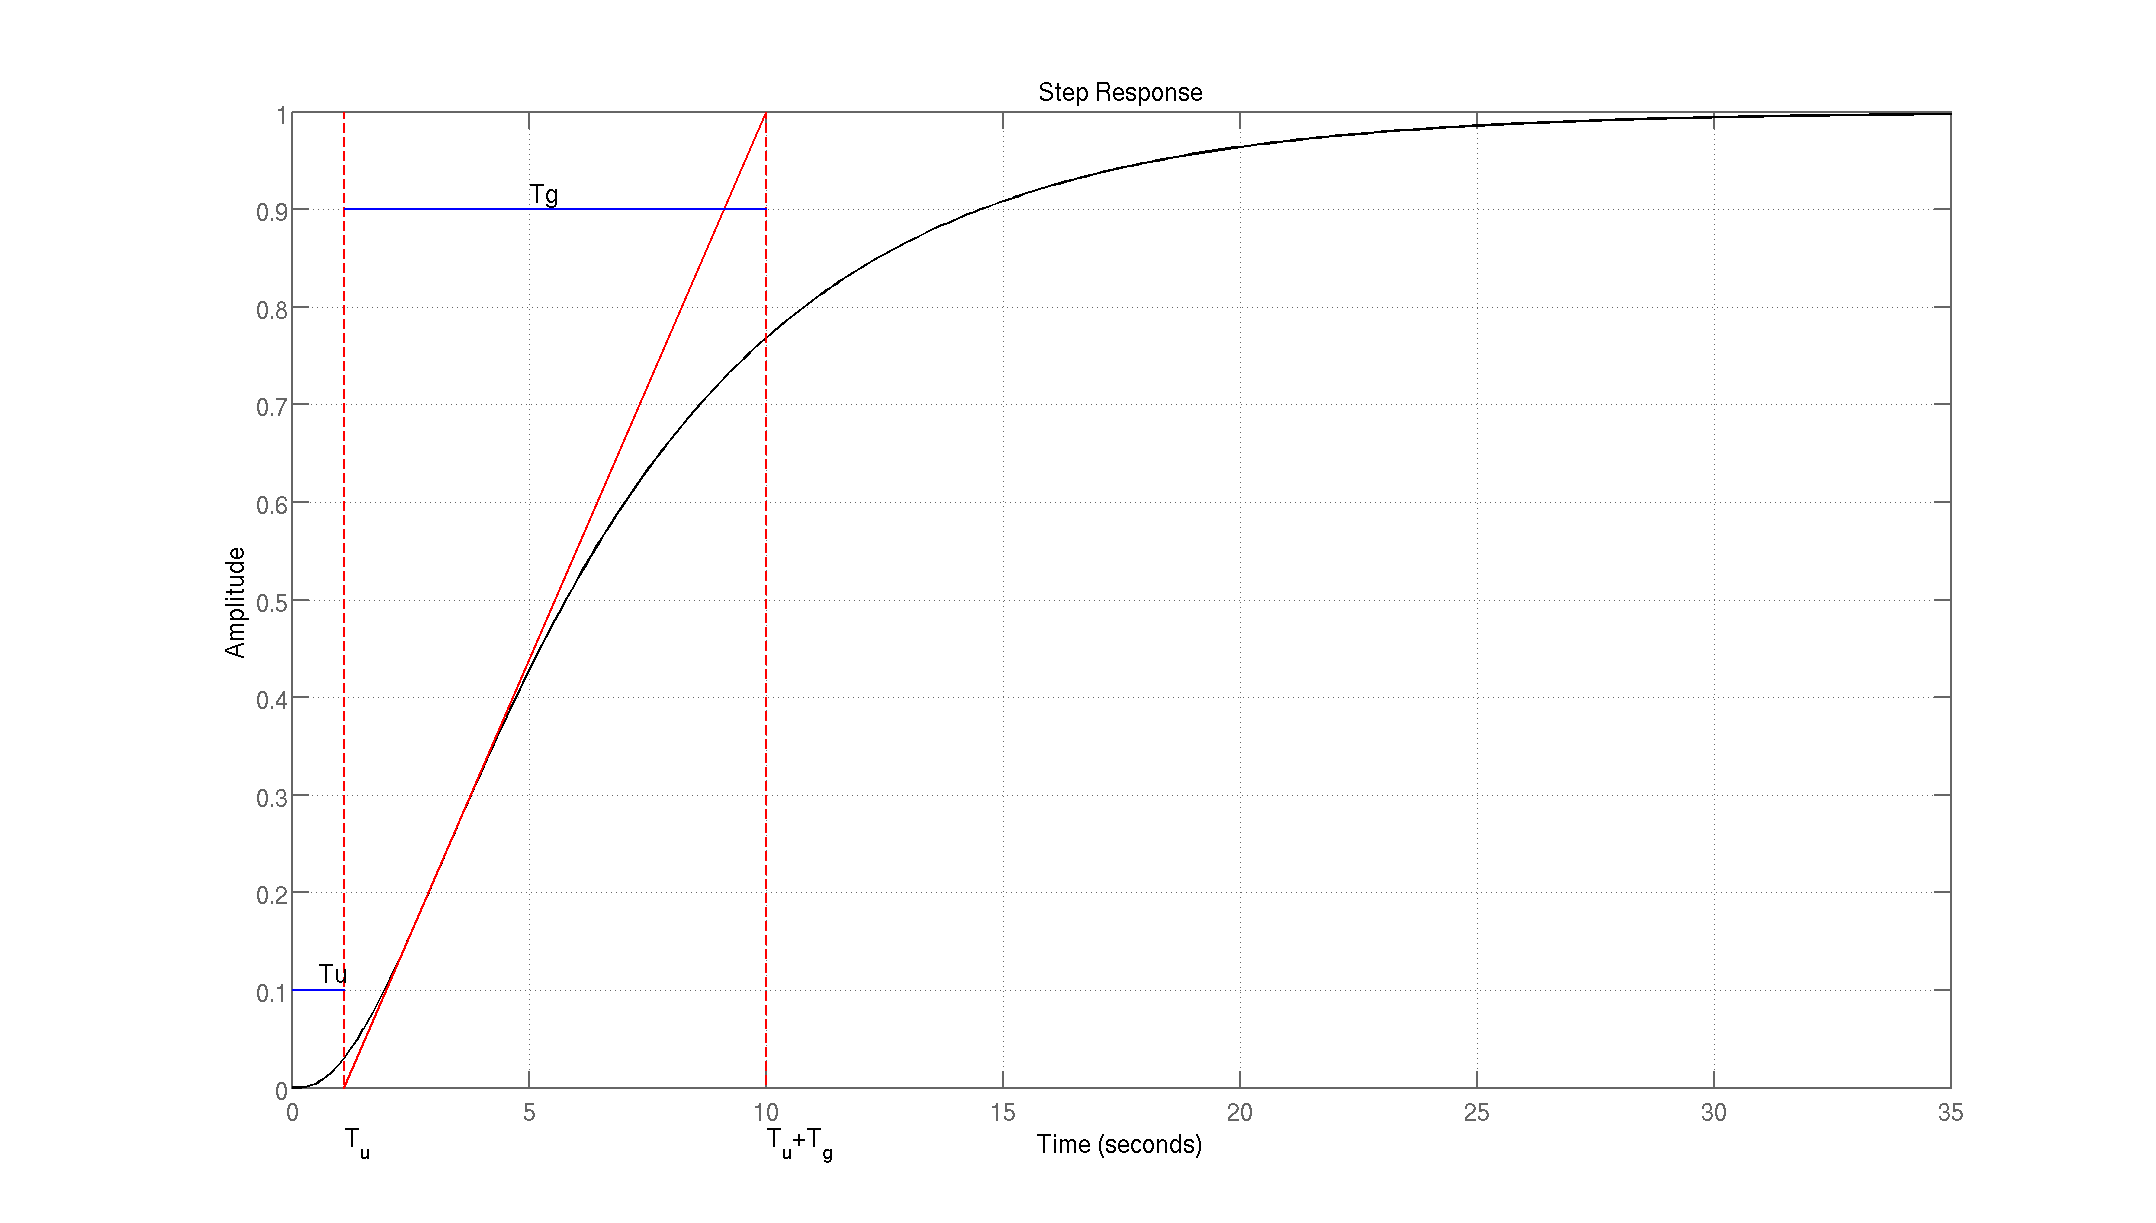
\includegraphics[width=\textwidth]{images/streckeSchrittantwort.png}
    \caption{%
    Schrittantwort der  Beispielstrecke (schwarz), Wendetangende  (rot), $T_u$
    und $T_g$ (blau)
    }
    \label{fig:plant_step}
\end{figure}

Ausmessen der Schrittantwort ergibt:
\begin{itemize}
    \item
        $K_s = 2$~\footnotemark[2]
    \item
        $T_u = \SI{1.1}{\second}$
    \item
        $T_g = \SI{8.9}{\second}$
\end{itemize}

\footnotetext[2]{%
    Abbildung~\ref{fig:plant_step}  ist  auf  1  normiert,  die  Verst\"arkung
    unserer  Beispielstrecke   betr\"agt  $2$.    An  den  Werten   f\"ur  die
    Verz\"ogerungs-  und Anstiegszeit  oder  am  Ausmessen der  Schrittantwort
    \"andert sich dadurch nichts
}

Der  geschlossene   Regelkreis  soll  schlussendlich  maximal   etwa  $16.3\%$
\"uberschwingen.

Da die Reglerdimensionierung mit der Phasengangmethode vom \emph{Frequenzgang}
einer   Strecke  ausgeht   und   nicht  von   deren  Schrittantwort,   besteht
der   n\"achste   Schritt    nun   darin,   aus   den    obigen   Werten   den
Frequenzgang   der   Strecke   zu   bestimmen. Dies   erledigt   die   Methode
\code{p\_sani}\footnotemark[3],    welche   uns    die    Werte   f\"ur    die
\"Ubertragungsfunktion  der  Strecke  liefert.
  In unserem  Fall ergibt
dies folgendes Polynom:

\footnotetext[3]{%
    Die  Methode  \code{p\_sani}  wurde  zu  Beginn  des  Projektes  in  einer
    Matlab-Implementation  zur Verf\"ugung  gestellt  und anschliessend  f\"ur
    unser Tool in Java \"ubersetzt.

    Sie kann aus der Verz\"ogerungszeit, der Anstiegszeit und der Verst\"arkung
    der Strecke ein Polynom f\"ur deren \"Ubertragungsfunktion vom Grad 1 bis 8
    ausrechnen.

    Als Eingabeparameter werden  die Werte $T_u$, $T_g$  und $K_s$ ben\"otigt,
    als R\"uckgabewert erh\"alt  man ein Array mit den Zeiten  $T_i$ f\"ur die
    Nenner der Faktoren des Polynoms (siehe Gleichung~\ref{eq:transfer:plant}).
}

\begin{gather} \label{eq:transfer:plant}
    \begin{split}
        H_s (s) & = K_s
                  \cdot \frac{1}{1 + s \cdot T_1}
                  \cdot \frac{1}{1 + s \cdot T_2}
                  \cdot \frac{1}{1 + s \cdot T_2}                     \\
                & = 2
                  \cdot \frac{1}{1 + s \cdot \SI{0.4134}{\second}}
                  \cdot \frac{1}{1 + s \cdot \SI{1.4894}{\second}}
                  \cdot \frac{1}{1 + s \cdot \SI{5.3655}{\second}}
    \end{split}
\end{gather}

Mit einem  geeigneten Tool  kann man sich  den dazugeh\"origen  Plot erstellen
lassen.

\begin{figure}[h! width=\pagewidth]
    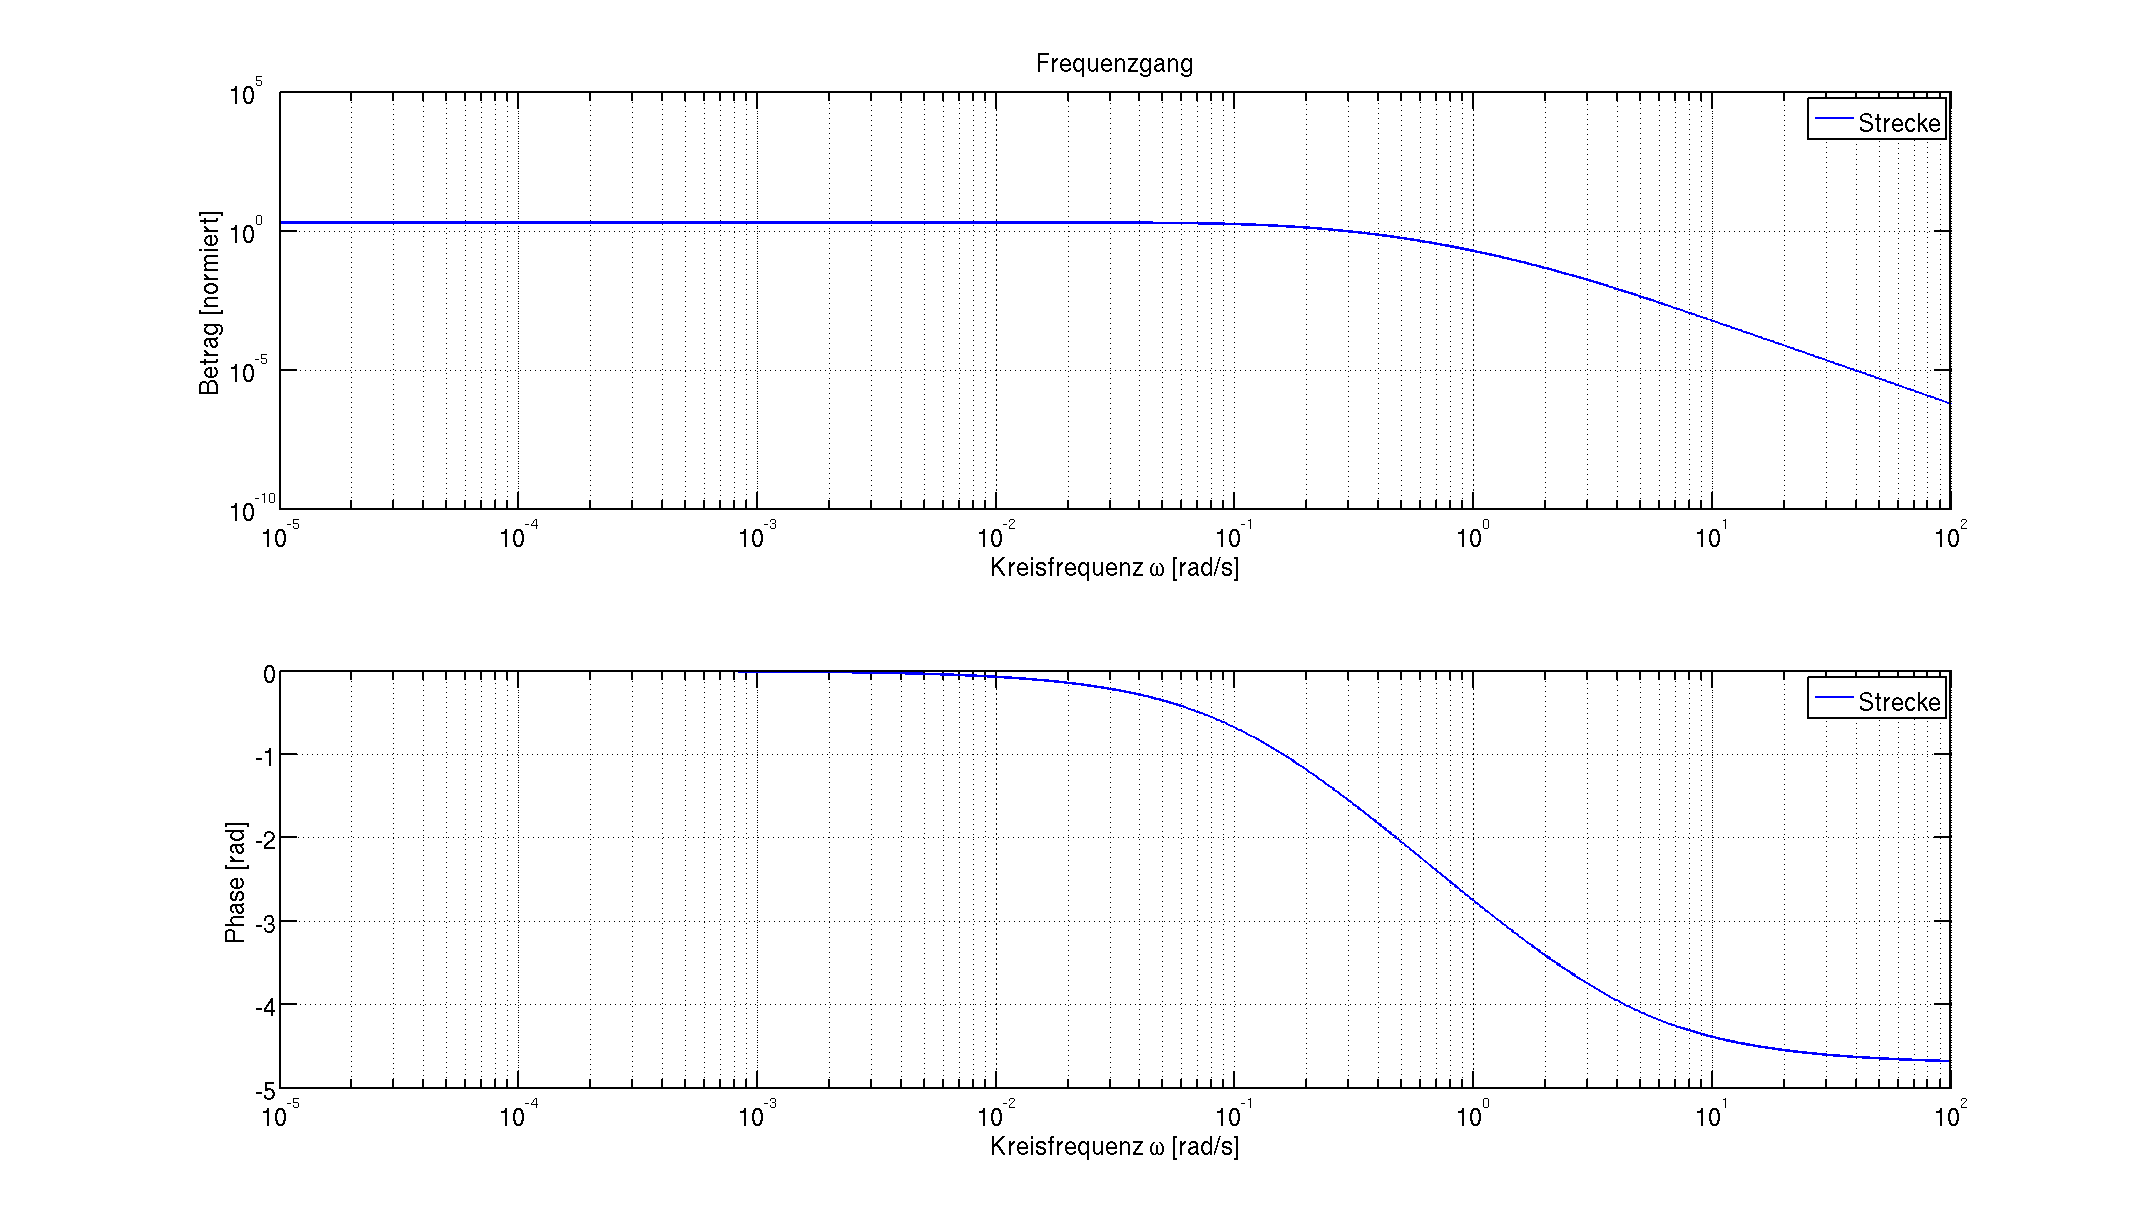
\includegraphics[width=\textwidth]{images/streckeFrequenzgang.png}
    \caption{%
        Frequenzgang der Strecke%
    }
    \label{fig:plant_freq}
\end{figure}

Somit  ist  der Frequenzgang  der  Strecke  bekannt  und  man kann  mit  einer
geeigneten Methode den Regler dimensionieren.


\clearpage
\subsection{Reglerdimensionierung mittels Faustformeln}
\label{subs:faustformeln}
Im   Praxiseinsatz  stehen   f\"ur   die  Dimensieung   der  Regler   einfache
Berechnungsformeln f\"ur die Einstellwerte der  Regler anhand von $T_u$, $T_g$
und $K_s$ zur Verf\"ugung.

Einige   dieser  Faustformeln   werden  in   der  Applikation   zum  Vergleich
mitberechnet. Die    dazugeh\"origen    Berechnungen    sind    der    Tabelle
\ref{tab:faustformeln} zu entnehmen.

\begin{longtable}{p{50mm}rrrrr}
    \toprule

    %\multicolumn{3}{l}{\large{\textsc{Auftragsanalyse und Hintergrundinformationen}}} \\

    Faustformel
    &
    \multicolumn{2}{l}{PI-Regler}
    &
    \multicolumn{2}{l}{PID-T1-Regler}
    \\

    &
    $T_n$
    &
    $K_p$
    &
    $T_n$
    &
    $T_v$
    &
    $K_p$
    \\

    \midrule

    \endhead
    \endfoot
    \endlastfoot

    % CONTENT HERE ---------------------------------------------------------- %

    \pbox{45mm}{Chiens, Hrones, Reswick \\ \small{\textbf{(0\% \"Uberschwingen)}} \\ \cite{ref:chiens_tsn}, \cite{ref:chiens_wiki}}
    &
    $1.2\cdot T_g$
    &
    $\frac{0.35}{K_s} \cdot \frac{T_g}{T_u}$
    &
    $T_g$
    &
    $0.5\cdot T_u$
    &
    $ \frac{0.6}{K_s} \cdot \frac{T_g}{T_u} $
    \\

    \addlinespace[1em]

    \pbox{45mm}{Chiens, Hrones, Reswick \small{\textbf{(20\% \"Uberschwingen)}} \\ \cite{ref:chiens_tsn}, \cite{ref:chiens_wiki}}
    &
    $T_g$
    &
    $\frac{0.6}{K_s} \cdot \frac{T_g}{T_u}$
    &
    $1.35\cdot T_g$
    &
    $0.47 \cdot T_u$
    &
    $ \frac{0.95}{K_s} \cdot \frac{T_g}{T_u} $
    \\

    \addlinespace[1em]

    Oppelt \cite{ref:op_ros_zieg}
    &
    $3 \cdot T_u$
    &
    $\frac{0.8}{K_s} \cdot \frac{T_g}{T_u}$
    &
    $2 \cdot T_u$
    &
    $ 0.42 \cdot T_u $
    &
    $ \frac{1.2}{K_s} \cdot \frac{T_g}{T_u} $
    \\

    \addlinespace[1em]

    Rosenberg \cite{ref:op_ros_zieg}
    &
    $3.3 \cdot T_u $
    &
    $ \frac{0.91}{K_s} \cdot \frac{T_g}{T_u} $
    &
    $ 2 \cdot T_u $
    &
    $ 0.45 \cdot T_u $
    &
    $ \frac{1.2}{T_s} \cdot \frac{T_g}{T_u}$
    \\

    \addlinespace[1em]

    Ziegler/Nichols \cite{ref:op_ros_zieg}
    &
    $ 3.33 \cdot T_u $
    &
    $ \frac{0.9}{K_s} \cdot \frac{T_g}{T_u} $
    &
    $ 2 \cdot T_u $
    &
    $ 0.5 \cdot T_u $
    &
    $ \frac{1.2}{K_s} \cdot \frac{T_g}{t_u} $
    \\

    \bottomrule
\caption{Faustformeln zur Reglerdimensionierung}
\label{tab:faustformeln}
\end{longtable}
\todo{Quellen hinzuf\"ugen}


\clearpage
\subsection{Reglerdimensionierung mittels Phasengangmethode: PI-Regler}
\label{subs:phasengang:pi}
Es  werden nun  anhand  der  Phasengangmethode sowohl  ein  PI-  wie auch  ein
PID-Regler f\"ur die in Abschnitt~\ref{subs:frequenzgang} ausgemessene Strecke
dimensioniert (siehe n\"achster Abschnitt f\"ur PID-Regler).

Tabelle~\ref{tab:terms}  fasst  die  h\"aufig verwendeten  Begriffe  in  einer
\"Ubersicht zusammen:

\begin{longtable}{lp{60mm}}
    \toprule
    \endhead
    \endfoot
    \endlastfoot

    % CONTENT HERE ---------------------------------------------------------- %

    $H_s(j\omega)                                                                   $ &  \"Ubertragungsfunktion der Regelstrecke \\
    $A_s(j\omega)=|H_s(j\omega)|                                                    $ &  Amplitudengang der Regelstrecke \\
    $\varphi_s(j\omega)=arg(H_s(j\omega))                                           $ &  Phasengang der Regelstrecke \\
    $H_r(j\omega)                                                                   $ &  \"Ubertragungsfunktion des Reglers \\
    $A_r(j\omega)=|H_r(j\omega)|                                                    $ &  Amplitudengang des Reglers \\
    $\varphi_r(j\omega)=arg(H_r(j\omega))                                           $ &  Phasengang des Reglers \\
    $H_o(j\omega)=H_s \cdot H_r(j\omega)                                            $ &  \"Ubertragungsfunktion des offenen Regelkreises \\
    $A_o(j\omega)=|H_o(j\omega)|                                                    $ &  Amplitudengang des offenen Regelkreises \\
    $\varphi_o(j\omega)=arg(H_o(j\omega))=\varphi_s(j\omega)+\varphi_r(j\omega)     $ &  Phasengang des offenen Regelkreises \\
    $H_{rpid}= K_{rk}\Big[ \frac{(1+sT_{nk})(1+sT_{vk})}{sT_{nk}}\Big]              $ & \"Ubertragungsfunktion des PID-Reglers \\
    $H_{rpi} = K_{rk}\Big[ 1 + \frac{1}{sT_{nk}} \Big]                              $ & \"Ubertragungsfunktion des PI-Reglers \\

    \bottomrule
    \caption{Die wichtigsten Begriffsdefinitionen}
    \label{tab:terms}
\end{longtable}


% ---------------------------------------------------------------------------- %
\subsubsection*{Ziel}
% ---------------------------------------------------------------------------- %
Das  Ziel dieses  Abschnittes ist  die Bestimmung  der Parameter  $K_{rk}$ und
$T_{nk}$ in der \"Ubertragungsfunktion des Reglers:

\begin{equation} \label{eq:pi:target}
    H_{rpi} = K_{rk} \cdot \biggl[ 1 + \frac{1}{s \cdot T_{nk}} \biggr]
\end{equation}


% ---------------------------------------------------------------------------- %
\subsubsection{Bestimmung der Reglerfrequenz $\mathbf{\boldsymbol{\omega}_{pi}}$}
% ---------------------------------------------------------------------------- %

Zuerst  wird im  Phasengang der  Strecke gem\"ass  Gleichung~\ref{eq:pi:phi_s}
die     Frequenz     $\omega_{pi}$      bestimmt,     f\"ur     welche     die
Phase     der    Strecke     $-90\degree$     betr\"agt,    ersichtlich     in
Abbildung~\ref{fig:pi:omega_pi}\footnotemark[4].

\begin{equation} \label{eq:pi:phi_s}
    \varphi_s(\omega_{pi}) = -90 \degree
\end{equation}

\footnotetext[4]{%
    Der  Winkel  stellt  keinen   endg\"ultigen  Wert  dar. Dieser  wurde  von
    Jakob  Zellweger  fixiert, um  eine  graphische  Evaluation \"uberhaupt  zu
    erm\"oglichen. Durch Anpassung dieses Wertes kann je nach Regelstrecke das
    Regelverhalten weiter optimiert werden.
}

\begin{figure}[h! width=\pagewidth]
    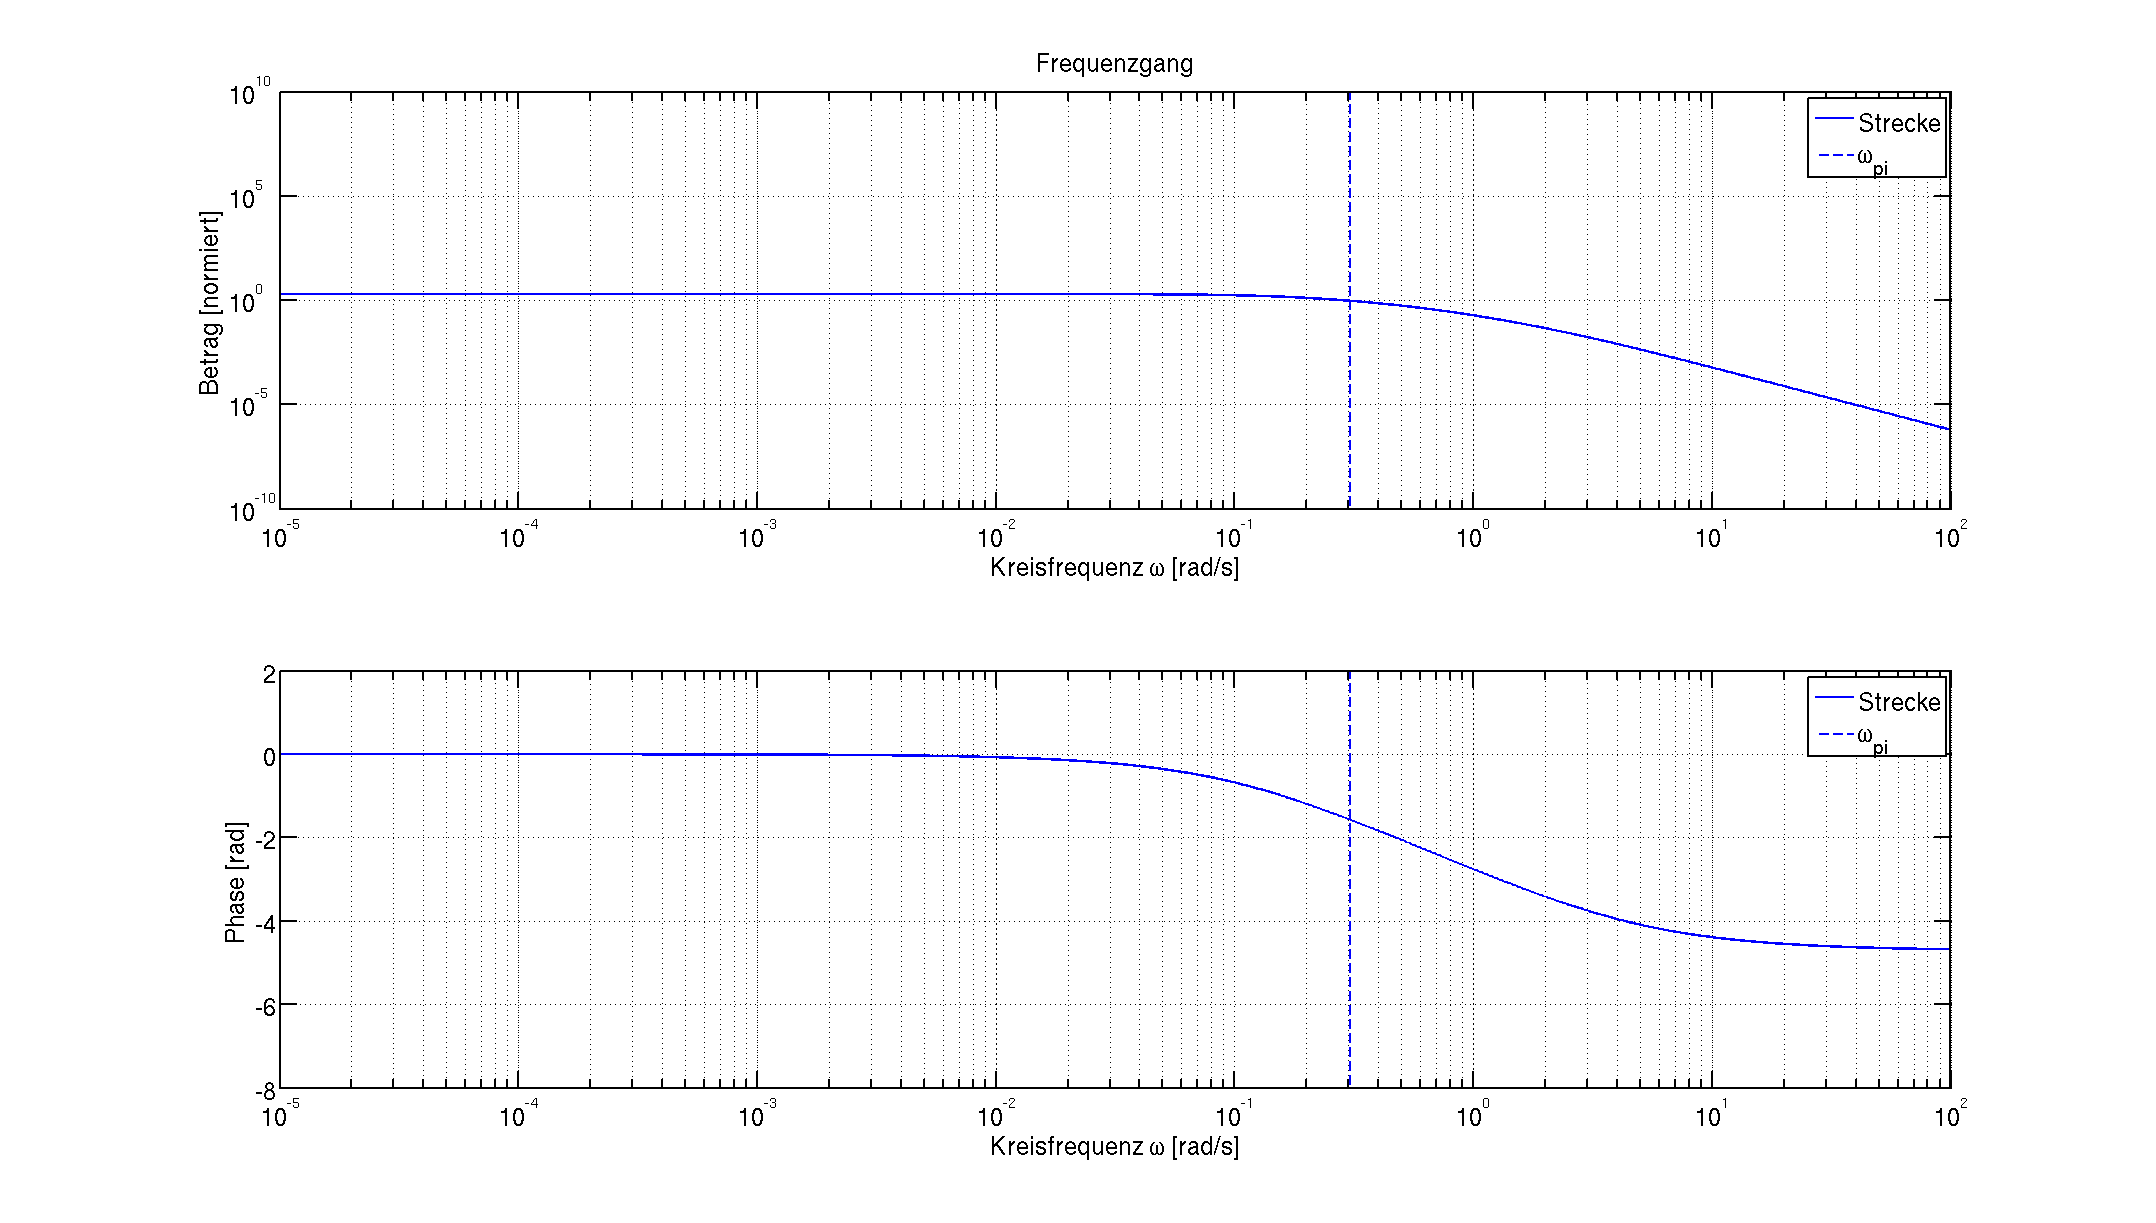
\includegraphics[width=\textwidth]{images/piStreckeOmegaPI.png}
    \caption{%
        Amplituden- und  Phasengang der Strecke mit  $\omega_{pi}$ eingetragen
        (vertikale gestrichelte Linie).
    }
    \label{fig:pi:omega_pi}
\end{figure}

Wie    man   aus    Abbildung~\ref{fig:pi:omega_pi}   ablesen    kann,   liegt
dieser   Wert  f\"ur   $\omega_{pi}$  in   unserem  Beispiel   bei  ungef\"ahr
$\SI{0.3}{\per\second}$. Die Kontrollrechnung mittels Matlab ergibt:

\begin{equation} \label{eq:pi:omega_pi}
    \omega_{pi} = \SI{0.3039}{\per\second}
\end{equation}


% ---------------------------------------------------------------------------- %
\subsubsection{Bestimmung von $\mathbf{T_{nk}}$}
% ---------------------------------------------------------------------------- %
Damit kann nun $T_{nk}$ direkt berechnet werden\footnotemark[5]:

\begin{equation} \label{eq:pi:omega_pi}
    T_{nk} = \frac{1}{\omega_{pi}} = \frac{1}{\SI{0.3039}{\per\second}} = \SI{3.2902}{\second}
\end{equation}

\footnotetext[5]{%
    Um die  Akkumulation von Ungenauigkeiten  zu minimieren, werden bei diesen
    Berechnungen  die  genauen  Werte  aus  Matlab  verwendet  und  nicht  die
    gerundeten  Zwischenresultate,  was  zu   Abweichungen  zu  den  von  Hand
    berechneten Ergebnissen f\"uhren kann.
}


% ---------------------------------------------------------------------------- %
\subsubsection{Bestimmung der Durchtrittsfrequenz $\mathbf{\boldsymbol{\omega}_d}$}
% ---------------------------------------------------------------------------- %

Die   Durchtrittsfrequenz  ist   die   Frequenz,  bei   der  die   betrachtete
\"Ubertragungsfunktion $H(j\omega)$ eine Verst\"arkung von $\SI{0}{\decibel} =
1$  aufweist. In der  Phasengangmethode soll  sie so  festgelegt werden,  dass
der  offene  Regelkreis  Gleichung~\ref{eq:phi_o} erf\"ullt. Dabei  ist  f\"ur
$\varphi_s$, abh\"angig vom gew\"unschten \"Uberschwingverhalten, ein Wert aus
Tabelle~\ref{tab:phi_s} auszuw\"ahlen\footnotemark[6].  Nach dem Festlegen der
Durchtrittsfrequenz (in  unserem Beispiel werden wir  $16.3\%$ anstreben) wird
dann im n\"achsten Abschnitt die Verst\"arkung des Reglers noch angepasst.

\footnotetext[6]{%
    Die  Werte f\"ur  $\varphi_s$  aus  Tabelle~\ref{tab:phi_s} stellen  keine
    abschliessende  Auflistung dar  und  sind lediglich  als Anhaltspunkte  zu
    betrachten. Weicht das Verhalten des geschlossenen Regelkreises am Schluss
    zu stark  vom gew\"unschten  Ergebnis ab, besteht  durch die  Wahl anderer
    Werte f\"ur $\varphi_s$ die M\"oglichkeit weiterer Optimierung.
}

\begin{equation} \label{eq:phi_o}
    \varphi_o(\omega_d)=\varphi_s.
\end{equation}

\begin{longtable}{llll}
    \toprule
    \endhead
    \endfoot
    \endlastfoot

    % CONTENT HERE ---------------------------------------------------------- %

    \"Uberschwingen & 0\%              & 16.3\%           & 23.3\% \\
    $\varphi_s$        & $-103.7 \degree$ & $-128.5 \degree$ & $-135 \degree$ \\

    \bottomrule
    \caption{Werte f\"ur $\varphi_s$}
    \label{tab:phi_s}
\end{longtable}

Um    Gleichung~\ref{eq:phi_o}    auswerten     zu    k\"onnen,    wird    der
Phasengang   des   offenen   Regelkreises   ben\"otigt. Dazu   wird   der   in
Gleichung~\ref{eq:pi:omega_pi}    erhaltene    Wert    f\"ur    $T_{nk}$    in
die   \"Ubertragungsfunktion    des   Reglers   (Gleichung~\ref{eq:pi:target})
eingesetzt. $K_{rk}$  ist  noch  unbekannt,  hat aber  auf  die  Phase  keinen
Einfluss und wird somit vorerst einfach auf 1 gesetzt.

\begin{gather} \label{eq:pi:target:inserted}
    \begin{split}
        H_{rpi} & = K_{rk} \cdot \biggl[ 1 + \frac{1}{s \cdot T_{nk}} \biggr] \\
                & = 1      \cdot \biggl[ 1 + \frac{1}{s \cdot \SI{3.2902}{\second}} \biggr]
    \end{split}
\end{gather}

Daraus kann nun der Frequenzgang  $H_o$ des offenen Regelkreises identifiziert
werden.

\begin{gather} \label{eq:pi:h_open}
    \begin{split}
        H_o (s) & = H_{rpi} (s) \cdot H_s (s) \\
            & = \Biggl(
                    K_{rk} \cdot \biggl[ 1 + \frac{1}{s \cdot T_{nk}} \biggr]
                \Biggr)
                \cdot
                K_s
                \cdot
                \Biggl(
                        \frac{1}{1 + s \cdot T_1}
                  \cdot \frac{1}{1 + s \cdot T_2}
                  \cdot \frac{1}{1 + s \cdot T_2}
                \Biggr) \\
            & = \Biggl(
                    1 \cdot \biggl[ 1 + \frac{1}{s \cdot \SI{3.2902}{\second}} \biggr]
                \Biggr)
                \cdot
                2
                \cdot
                \Biggl(
                          \frac{1}{1 + s \cdot \SI{0.4134}{\second}}
                    \cdot \frac{1}{1 + s \cdot \SI{1.4894}{\second}}
                    \cdot \frac{1}{1 + s \cdot \SI{5.3655}{\second}}
                \Biggr)
    \end{split}
\end{gather}


Von   besonderem    Interesse   ist   der    Phasengang   $\varphi_o(j\omega)$
dieser   \"Ubertragungsfunktion. Wie  oben   festgelegt,  soll   ein  maximals
\"Uberschwingen  von   ca. $16.3\%$  angestrebt  werden. Dazu   muss  gem\"ass
Tabelle~\ref{tab:phi_s}  die Durchtrittsfrequenz  $\omega_d$ gefunden  werden,
an  welcher der  offene  Regelkreis eine  Phase  von $-128.5\degree$  aufweist
(Gleichung~\ref{eq:phi_o}). In   Abbildung~\ref{fig:pi:omega_d}   kann   diese
Beziehung graphisch verifiziert werden.

\begin{figure}[h! width=\pagewidth]
    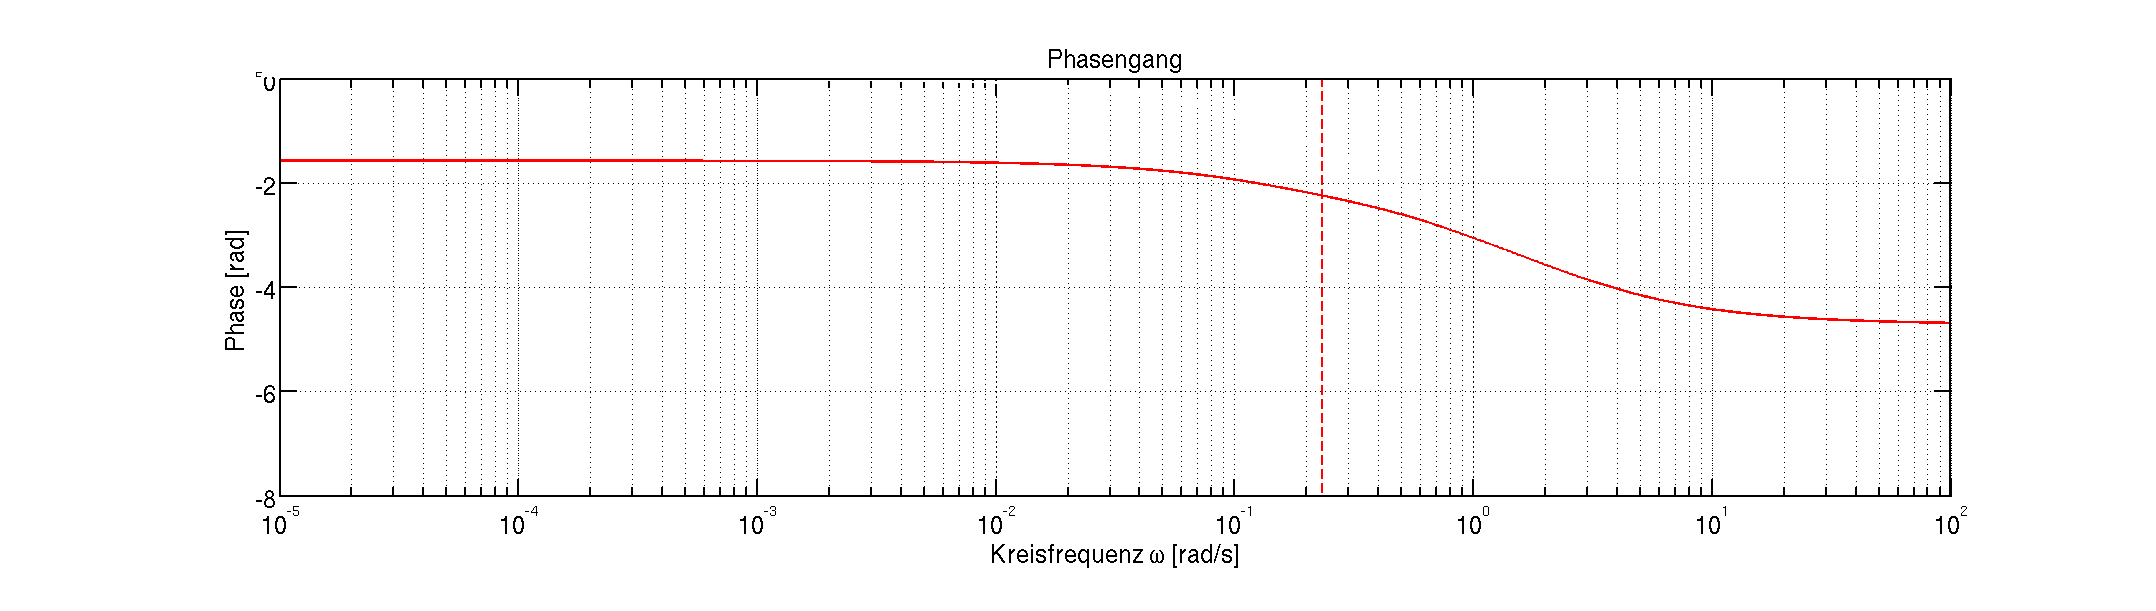
\includegraphics[width=\textwidth]{images/piOffenerRegelkreisPhasengang.png}
    \caption{%
        Phasengang   $\varphi_o(j\omega)$   des   offenen   Regelkreises   mit
        eingetragener Durchtrittsfrequenz $\omega_{d}$ (vertikale gestrichelte
        Linie). Wie man  sieht, weist der offene  Regelkreis unseres Beispiels
        bei dieser Kreisfrequenz eine Phase von $-128.5\degree$ auf
        (etwa $\SI{-2.24}{\radian}$).
    }
    \label{fig:pi:omega_d}
\end{figure}

Dies ergibt f\"ur die Durchtrittsfrequenz:
\begin{equation} \label{eq:pi:omega_d}
    \omega_d = \SI{0.2329}{\per\second}
\end{equation}


% ---------------------------------------------------------------------------- %
\subsubsection{Bestimmung der Reglerverst\"arkung $\mathbf{K_{rk}}$}
% ---------------------------------------------------------------------------- %

Im  letzten  Schritt  muss  nun, wie im  vorherigen  Abschnitt  erw\"ahnt, die
Verst\"arkung  $K_{rk}$   des  Reglers   noch  angepasst  werden,   damit  der
offene   Regelkreis  bei   der  angestrebten   Durchtrittsfrequenz  $\omega_d$
auch  effektiv  eine Verst\"arkung  von  1  aufweist.  Dazu  wird  $j\omega_d$
in  Gleichung~\ref{eq:pi:h_open}  f\"ur  den   Parameter  $s$  eingesetzt  und
$|H_o(j\omega_d)| = 1$ gesetzt.

\begin{gather} \label{eq:pi:A_o_set_to_one}
    \begin{split}
        A_o & = | H_o (j\omega_d) | = | H_{rpi} (j\omega) \cdot H_s (j\omega)| \\
            & = \abs*{
                    \bigg(
                        K_{rk} \cdot \biggl[ 1 + \frac{1}{j \cdot \omega_d \cdot T_{nk}} \biggr]
                    \bigg)
                    \cdot
                    K_s
                    \cdot
                    \bigg(
                            \frac{1}{1 + j \cdot \omega_d \cdot T_1}
                      \cdot \frac{1}{1 + j \cdot \omega_d \cdot T_2}
                      \cdot \frac{1}{1 + j \cdot \omega_d \cdot T_2}
                      \bigg)} \\
              & = 1
    \end{split}
\end{gather}

Mit den Werten
\begin{equation} \label{eq:pi:values}
    \begin{split}
        K_s      & = 2                    \\
        T_{nk}   & = \SI{3.2902}{\second} \\
        T_1      & = \SI{0.4134}{\second} \\
        T_2      & = \SI{1.4894}{\second} \\
        T_3      & = \SI{5.3655}{\second} \\
        \omega_d & = \SI{0.2329}{\radian\per\second}
    \end{split}
\end{equation}

l\"ost  man Gleichung  \ref{eq:pi:A_o_set_to_one}  nun nach  $K_{rk}$ auf  und
erh\"alt:

\begin{equation} \label{eq:pi:k_rk_result}
    K_{rk} = 0.517577
\end{equation}


% ---------------------------------------------------------------------------- %
\subsubsection{Resultat}
% ---------------------------------------------------------------------------- %

Somit ist der PI-Regler vollst\"andig bestimmt und hat folgende Form:

\begin{equation} \label{eq:pi:result}
    H_{rpi} = 0.518 \cdot \biggl[ 1 + \frac{1}{s \cdot \SI{3.29}{\second}} \biggr]
\end{equation}

In Abbildung~\ref{fig:pi:all} sind die  wichtigsten Werte f\"ur diesen Prozess
nochmals in einer \"Ubersicht zusammengefasst.

\begin{figure}[h! width=\pagewidth]
    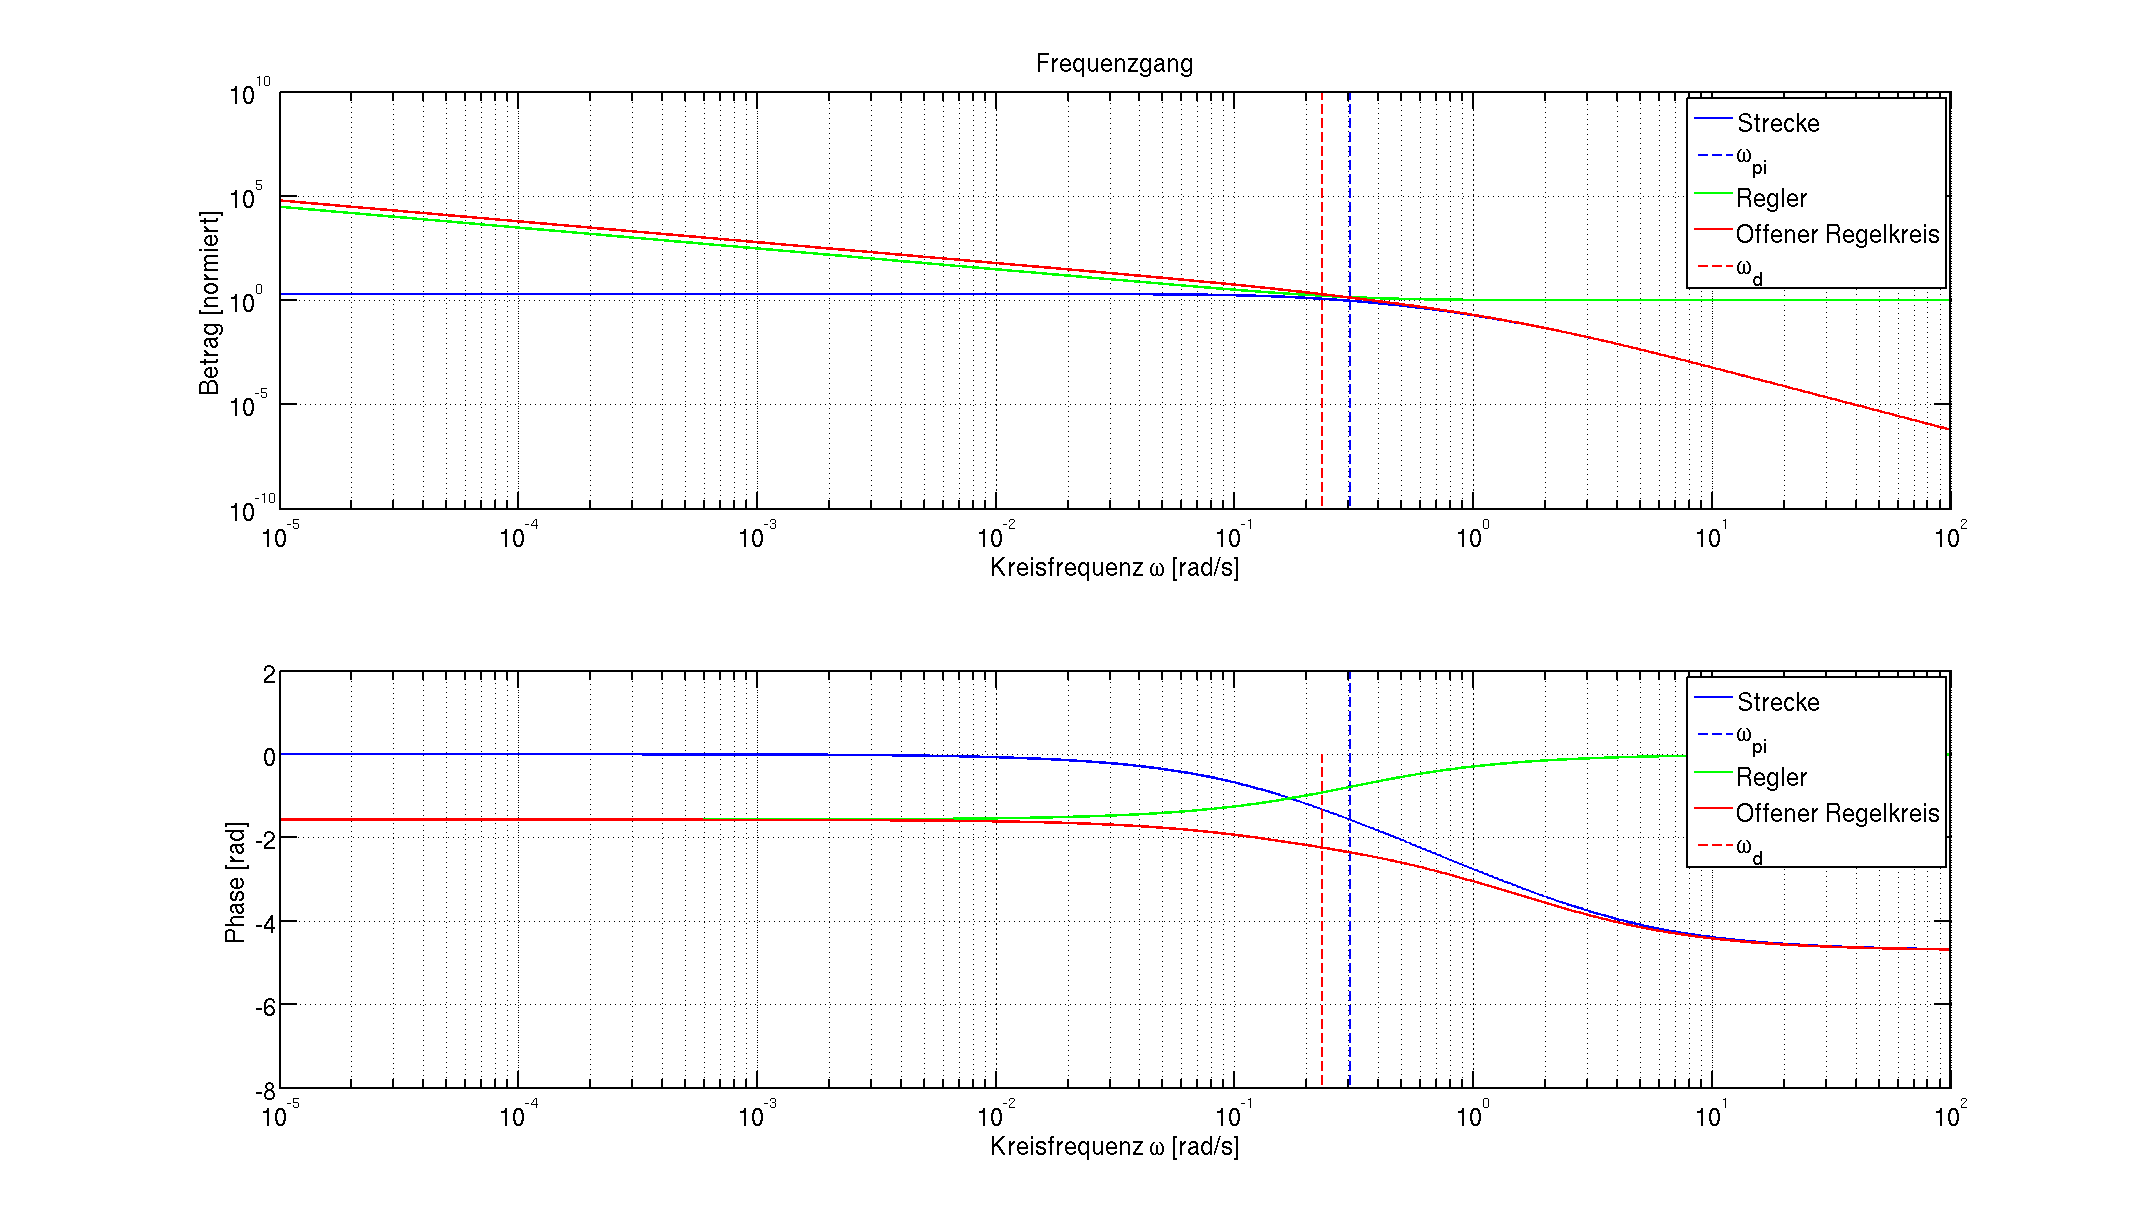
\includegraphics[width=\textwidth]{images/piBode.png}
    \caption{%
        Frequenzgang des Reglers (gr\"un), der  Strecke (blau) und des offenen
        Regelkreises (rot).
    }
    \label{fig:pi:all}
\end{figure}


\clearpage
\subsection{Reglerdimensionierung mittels Phasengangmethode: PID-Regler}
\label{subs:phasengang:pid}
\subsubsection*{Ziel}
Das Ziel ist  die Bestimmung der Parameter $K_{rk}$, $T_{nk}$  und $T_{vk}$ in
der Gleichung:

\begin{equation} \label{eq:pid:target}
    H_{rpid} = K_{rk} \cdot \biggl[ \frac{(1 + s \cdot T_{nk}) \cdot (1 + s \cdot T_{vk}) }{ s \cdot T_{nk} } \biggr]
\end{equation}


\subsubsection{Bestimmung der Reglerfrequenz $\omega_{pid}$}

Analog  zum PI-Regler  wird zuerst  im  Phasengang der  Strecke die  Frequenz
$\omega_{pid}$ bestimmt, f\"ur  welche die Phase der  Strecke einen bestimmten
Wert aufweist, nur wird hier $-135\degree$ benutzt:

\begin{equation} \label{eq:pid:phi_s}
    \varphi_s(\omega_{pid}) = -135 \degree
\end{equation}

In unserem Beispiel ergibt dies:

\begin{equation} \label{eq:pid:omega_pid}
    \omega_{pid} = \SI{0.6714}{\per\second}
\end{equation}


\subsubsection{Steigung des Phasengangs bei der Reglerfrequenz}

Anschliessend wird  die Steigung des  Phasengangs $\varphi_s$ der  Strecke bei
der  Frequenz  $\omega_{pid}$  bestimmt. Ausgangspunkt  daf\"ur  ist  die  von
\code{p\_sani} bestimmte  \"Ubertragungsfunktion der Strecke  (siehe Gleichung
\ref{eq:transfer:plant}).

\begin{equation} \label{eq:transfer:plant:derivative}
    \frac{d\varphi_s}{d\omega} \biggr \rvert_{\omega=\omega_{pid}}
        = \frac{d(arg(H_s(j\omega)))}{d\omega} \biggr \rvert_{\omega=\omega_{pid}}
        = \SI{-1.5124}{\second}
\end{equation}
\todo{Einheit \"uberpr\"ufen}


\subsubsection{Hilfsparameter $\beta$}

Zwischen den Steigungen der Phasen des offenen Regelkreises ($\varphi_o$), der
Strecke ($\varphi_s$) und des Reglers ($\varphi_r$) gilt folgende Beziehung:

\begin{equation} \label{eq:pid:phi_sum}
    \varphi_o = \varphi_s + \varphi_r
\end{equation}

Da die Ableitung eine lineare Funktion ist, gilt somit auch: \todo{korrekte Begriffe}
\begin{equation} \label{eq:pid:dphi_sum}
    \frac{d\varphi_o}{d\omega} = \frac{d\varphi_s}{d\omega} + \frac{d\varphi_r}{d\omega}
\end{equation}

Diese Beziehungen  k\"onnen auch  gut in Abbildung  \ref{fig:pid_complete} von
Hand \"uberpr\"uft werden.

Es soll nun gelten:

\begin{equation} \label{eq:pid:dphi_o_target}
    \frac{d\varphi_o}{d\omega} \biggr \rvert_{\omega=\omega_{pid}} = - \frac{1}{2}
\end{equation}

Da   $\frac{d\varphi_s}{d\omega}$  durch   die  Strecke   gegeben  und   somit
unver\"anderlich ist, kann lediglich der Wert von $\frac{d\varphi_r}{d\omega}$
angepasst     werden,     damit     $\frac{d\varphi_o}{d\omega}$     Gleichung
\ref{eq:pid:dphi_o_target} erf\"ullt.

Dazu f\"uhrt man den Hilfsparameter $\beta$ ein, f\"ur den gilt:

\begin{gather} \label{eq:pid:beta:start}
    \begin{split}
        \frac{1}{T_{vk}} & = \frac{\omega_{pid}}{\beta} \\
        \frac{1}{T_{nk}} & = \omega_{pid} \cdot \beta  \\
                       0 & <  \beta \leq 1
    \end{split}
\end{gather}

Die  beiden Frequenzen  $\frac{1}{T_{vk}}$  und  $\frac{1}{T_{nk}}$ sind  also
symmetrisch  um den  Faktor $\beta$  gr\"osser bzw.  kleiner als  die Frequenz
$\omega_{pid}$. \todo{siehe Plot} Will man  $\beta$ von Hand bestimmen, trifft
man zuerst eine ``vern\"unftige'' Annahme, zum Beispiel:

\begin{equation} \label{eq:pid:beta:initial_value}
    \beta = 0.5
\end{equation}

Mit  diesem Startwert  bestimmt  man nun  $T_{nk}$  und ${T_{vk}}$. Die  somit
erhaltenen Werte setzt man in  Gleichung \ref{eq:pid:target} ein, zusammen mit
dem Wert f\"ur $\omega_{pid}$ aus Gleichung \ref{eq:pid:omega_pid}:

\begin{gather} \label{eq:pid:t_nk_t_vk_initial_results}
    \begin{split}
        {T_{vk}} & = \frac{\beta}{\omega_{pid}}  = \frac{0.5}{\SI{0.6714}{\per\second}}                   = \SI{0.7447}{\second} \\
        {T_{nk}} & = \frac{1}{\omega_{pid} \cdot \beta} = \frac{1}{\SI{0.6714}{\per\second} \cdot 0.5 }  = \SI{2.9789}{\second} \\
    \end{split}
\end{gather}

Eingesetzt in die Reglergleichung, vorerst mit $K_{rk} = 1$:

\begin{gather} \label{eq:pid:t_nk_t_vk_initial_results}
    \begin{split}
        H_{rpid} & = K_{rk} \cdot \biggl[ \frac{(1 + j\omega \cdot T_{nk}) \cdot (1 + j\omega \cdot T_{vk}) }{ j\omega \cdot T_{nk} } \biggr] \\
                 & = 1      \cdot \biggl[ \frac{(1 + j\omega \cdot \SI{2.9789}{\second}) \cdot (1 + j\omega \cdot \SI{0.7447}{\second}) }{ j\omega \cdot  \SI{2.9789}{\second}} \biggr]
    \end{split}
\end{gather}

Von dieser Gleichung bestimmt man nun den Phasengang und wertet danach dessen
Ableitung an der Stelle $\omega = \omega_{pid}$ aus:

\begin{gather} \label{eq:pid:phi_r_first_iteration}
    \begin{split}
        \varphi_s (j\omega)                                            & = arg(H_{rpid}(j\omega))        \\
        \frac{d\varphi_s}{d\omega} \biggr \rvert_{\omega=\omega_{pid}} & = \SI{1.1920}{\second}
    \end{split}
\end{gather}
\todo{Die zugeh\"orige Rechnung ist lange und m\"uhsam, allenfalls in Anhang? Ebenfalls: Einheit kontrollieren}


Setzt man dies in Gleichung \ref{eq:pid:phi_sum} ein, erh\"alt man:
\begin{gather} \label{eq:pid:phi_sum_result_iteration_one}
    \begin{split}
    \frac{d\varphi_o}{d\omega}       \biggr \rvert_{\omega=\omega_{pid}, \beta=0.5}
        & = \frac{d\varphi_s}{d\omega} \biggr \rvert_{\omega=\omega_{pid}}
        + \frac{d\varphi_r}{d\omega} \biggr \rvert_{\omega=\omega_{pid}, \beta=0.5} \\
        & = \SI{-1.5124}{\second} + \SI{1.1920}{\second} \\
        & = \SI{-0.3204}{\second} \\
        & > -\frac{1}{2}
    \end{split}
\end{gather}

Mit  $\beta  = 0.5$  erh\"alt  man  also eine  zu  hohe  Steigung des  offenen
Regelkreises   an    der   Stelle  $\omega_{pid}$,   folglich   muss   $\beta$
{\em{verkleinert}} werden.   Diese Berechnungen  werden nun mit  jeweils neuen
Werten  f\"ur  $\beta$  solange  wiederholt,  bis  die  Steigung  des  offenen
Regelkreises die gew\"unschte N\"ahe zu $-\frac{1}{2}$ aufweist.

Da die manuelle Iterierung dieses Prozesses enorm viel Zeit in Anspruch nimmt,
bietet  sich  hier  eine  Automatisierung  an. Die  Berechnung  mittels  eines
geeigneten Algorithmus in Matlab liefert schlussendlich folgendes Ergebnis:
\todo{Allenfalls Matlab-Algo in Anhang und Verweis}

\begin{gather} \label{eq:pid:beta_result}
    \begin{split}
        \beta    & = 0.2776 \\
        {T_{vk}} & = \frac{\beta}{\omega_{pid}}           = \SI{0.4134}{\second} \\
        {T_{nk}} & = \frac{1}{\omega_{pid} \cdot \beta}   = \SI{5.3656}{\second} \\
    \end{split}
\end{gather}

Sollte  man  f\"ur  $\beta$  einen komplexen  Wert  erhalten,  wird  $\beta=1$
gesetzt.\todo{Wie kann dies egtl. passieren?}


\subsubsection{Durchtrittsfrequenz $\omega_d$}

Diese  Werte setzt man nun in Gleichung \ref{eq:pid:target} ein. $K_{rk}$ wird
wie bei der Bestimmung von $\beta$ vorerst noch auf 1 gesetzt.

\begin{gather} \label{eq:pid:h_rpid_beta_result}
    \begin{split}
        H_{rpid} & = K_{rk} \cdot \biggl[ \frac{(1 + s \cdot T_{nk}               ) \cdot (1 + s \cdot T_{vk}               ) }{ s \cdot T_{nk}               } \biggr]
                   = 1      \cdot \biggl[ \frac{(1 + s \cdot \SI{5.3656}{\second} ) \cdot (1 + s \cdot \SI{0.4134}{\second} ) }{ s \cdot \SI{5.3656}{\second} } \biggr]
    \end{split}
\end{gather}

Zur Bestimmung von $K_{rk}$ wird nun der Frequenzgang des offenen Regelkreises
betrachtet. Dazu  multipliziert  man  wie  gehabt  die  \"Ubertragungsfunktion
der  Strecke   (siehe  Gleichung   \ref{eq:transfer:plant})  mit   der  soeben
bestimmten  provisorischen   \"Ubertragungsfunktion  des   Reglers  (Gleichung
\ref{eq:pid:h_rpid_beta_result}).

\begin{equation} \label{eq:pid:h_o_k_rk_one}
    H_{o}(j\omega) = H_{rpid}(j\omega) \cdot H_s(j\omega)
\end{equation}

Nun wird  die Durchtrittsfrequenz $\omega_d$  bestimmt, an welcher  der offene
Regelkreis eine  Verst\"arkung von $\SI{0}{\decibel} =  1$ aufweisen soll. Wie
auch  beim  PI-Regler  werden  wir   hier  ein  \"Uberschwingen  von  $16.3\%$
anstreben, womit gem\"ass Tabelle \ref{tab:phi_s}gilt:

\begin{equation} \label{eq:pid:omega_d_target}
    \varphi_s(\omega_d) = \varphi_s = -128.5\degree
\end{equation}

Dieser Wert wird analog zum PI-Regler aus dem Phasengang des offenen Regelkreises
abgelesen. \todo{siehe Plot} Eine Nachrechnung mittels Matlab ergibt:


\begin{equation} \label{eq:pid:omega_d_target}
    \omega_d = \SI{0.5341}{\per\second}
\end{equation}


\subsubsection{Bestimmung der Reglerverst\"arkung $K_{rk}$}

In einem letzten Schritt wird  nun der Amplitudengang des offenen Regelkreises
an der  Stelle $\omega_d$ gleich 1  gesetzt und diese Gleichung  nach $K_{rk}$
aufgel\"ost:

\begin{equation} \label{eq:pid:h_o_k_rk_one}
    \begin{split}
        A_{o}(j\omega_d)    & = | H_{o}(j\omega_d) |                            \\
                            & = | H_{rpid}(j\omega_d) \cdot H_s(j\omega_d) |    \\
                            & = \Biggl \rvert
                                    K_{rk}
                                    \cdot
                                    \biggl[ \frac{(1 + j\omega_d \cdot T_{nk}) \cdot (1 + j\omega_d \cdot T_{vk}) }{ j\omega_d \cdot T_{nk} } \biggr] \Biggr \rvert \\
                            & \cdot
                                \Biggl \rvert
                                    K_s
                                    \cdot \frac{1}{1 + j\omega_d \cdot T_1}
                                    \cdot \frac{1}{1 + j\omega_d \cdot T_2}
                                    \cdot \frac{1}{1 + j\omega_d \cdot T_2}
                                    \Biggr \rvert \\
                            & = 1
    \end{split}
\end{equation}

Mit den gegebenen und berechneten Werten:
\begin{gather} \label{eq:pid:h_o_k_rk_one}
    \begin{split}
        K_s         & = 2                        \\
        T_1         & = \SI{0.4134}{\second}     \\
        T_2         & = \SI{1.4894}{\second}     \\
        T_3         & = \SI{5.3655}{\second}     \\
        T_{nk}      & = \SI{5.3656}{\second}     \\
        T_{vk}      & = \SI{0.4134}{\second}     \\
        \omega_d    & = \SI{0.5341}{\per\second}
    \end{split}
\end{gather}

Dies liefert:

\begin{equation} \label{eq:pid:k_rk_result}
    K_{rk} = 1.83084
\end{equation}


\subsubsection{Resultat}

Somit ist der Regler vollst\"andig bestimmt und hat folgende \"Ubertragungsfunktion:

\begin{equation} \label{eq:pid:result}
    H_{rpid}(s) = 1.83084 \cdot \biggl[ \frac{(1 + s \cdot \SI{5.3656}{\second} ) \cdot (1 + s \cdot \SI{0.4134}{\second} ) }{ s \cdot \SI{5.3656}{\second} } \biggr]
\end{equation}

Die Frequenzg\"ange der Strecke, des Reglers und des offenen Regelkreises:

\begin{figure}[h! width=\pagewidth]
    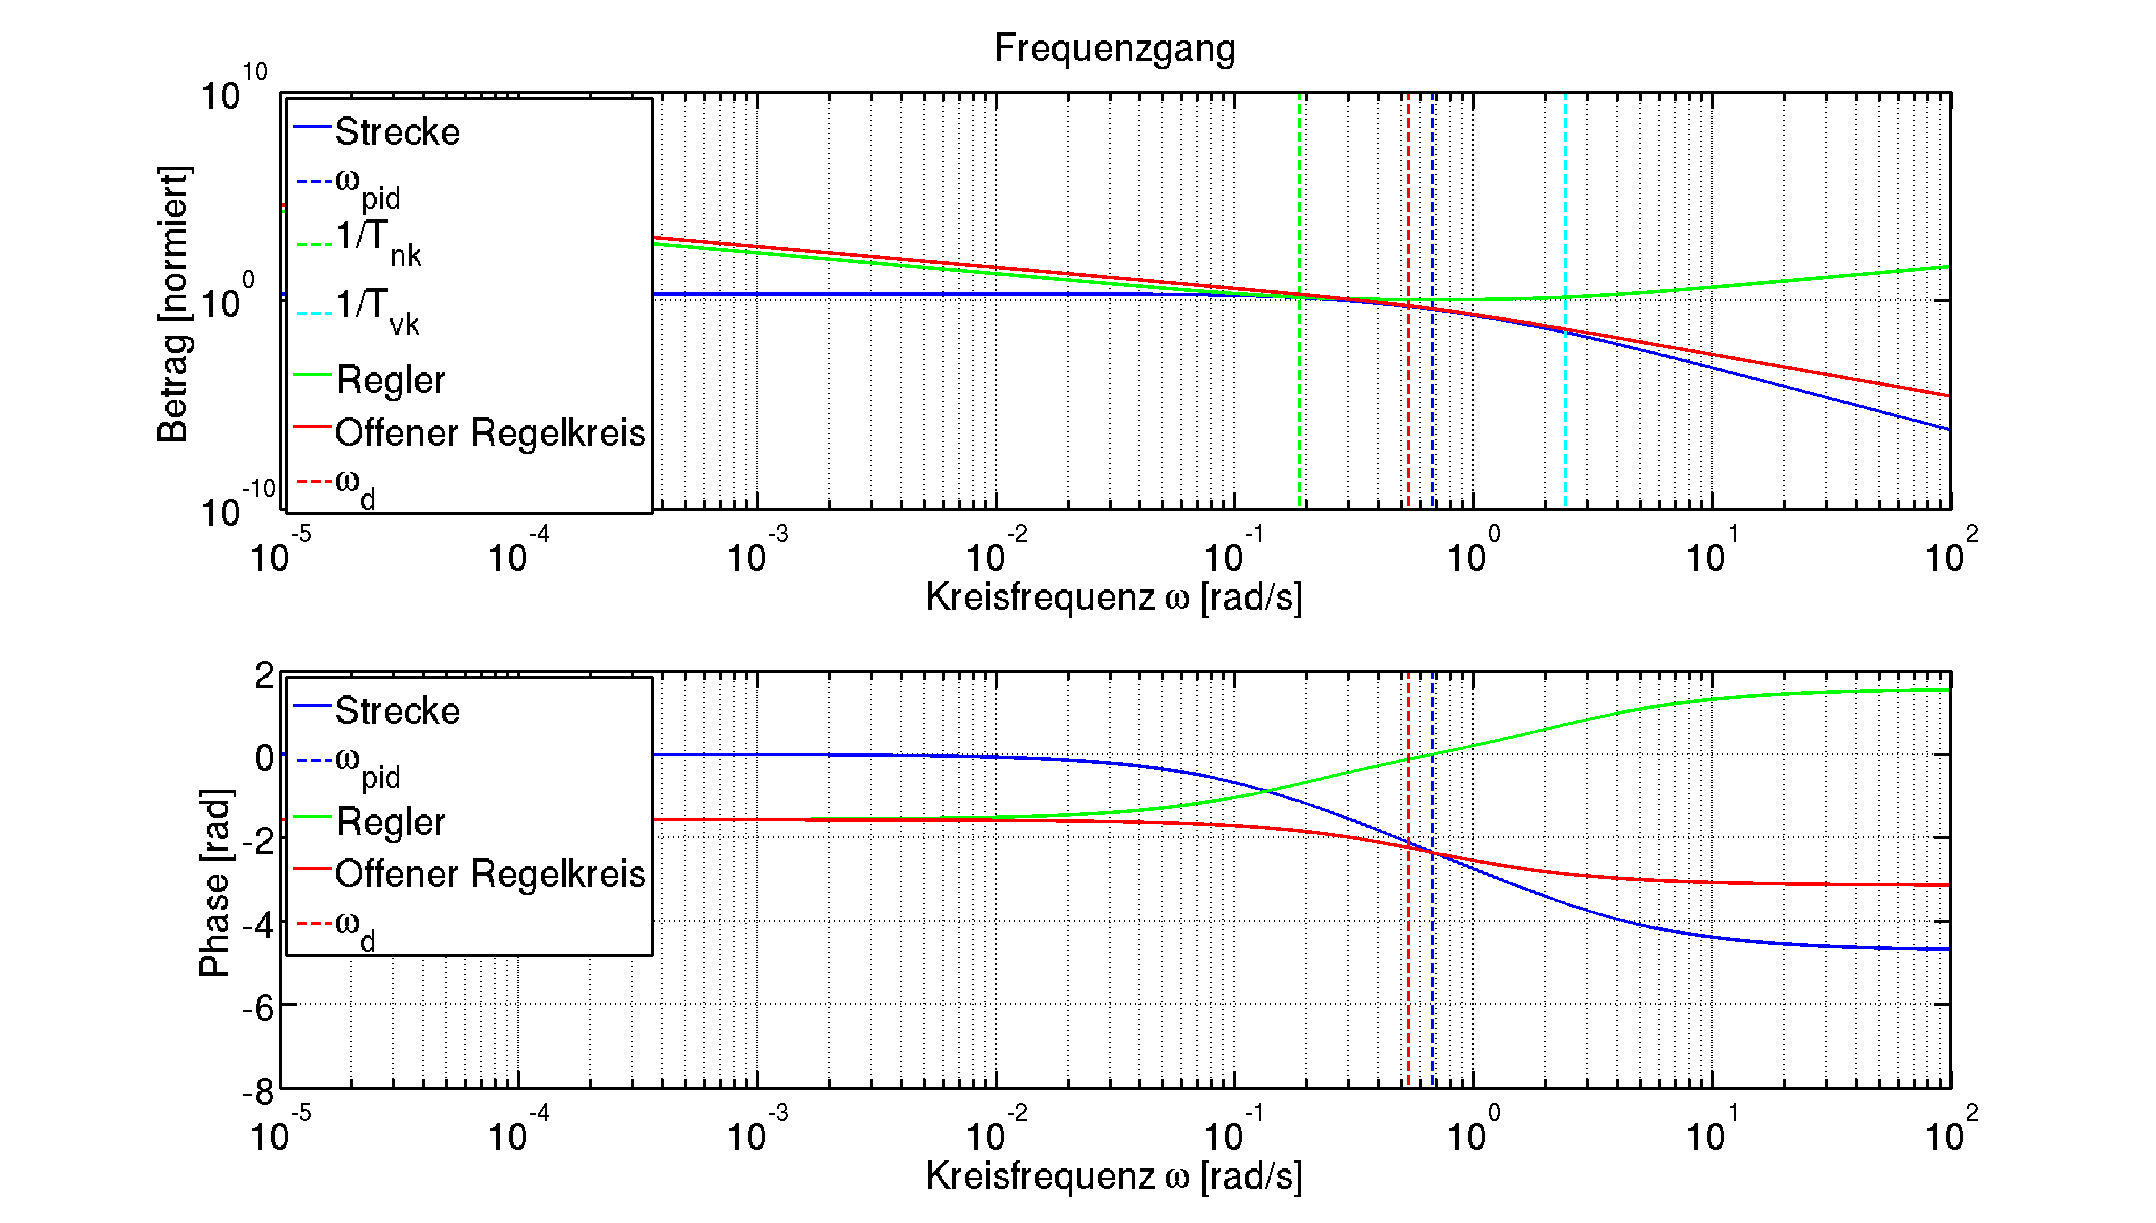
\includegraphics[width=\textwidth]{images/pidCompletePlot.png}
    \caption{%
        Frequenzgang der Strecke (blau), des  Reglers (gr\"un) und des offenen
        Regelkreises  (rot).  Ebenfalls  eingetragen  sind die  Reglerfrequenz
        $\omega_{pid}$,   die   beiden   Frequenzen   $\frac{1}{T_{vk}}$   und
        $\frac{1}{T_{nk}}$ sowie die Durchtrittsfrequenz $\omega_d$.
    }
    \label{fig:pid_complete}
\end{figure}
\clearpage


\clearpage
\subsection{Vergleich mit Software-Tool}
\label{subs:tool:results}
Zum  Vergleich  mit  den  soeben  dimensionierten  PI-  und  PID-Reglern  sind
hier   noch  die   Resultate   der  Dimensionierung   mittels  unseres   Tools
gezeigt. Wie  zu erwarten  weisen die  mit  dem Tool  berechneten Werte  f\"ur
die  Faustformeln   keine  signifikanten  Abweichenungen  zu   den  Werten  in
Tabelle~\ref{tab:ff_results} auf.

Verwendet man  in den Berechnungen mittels  Phasengangmethode den Standardwert
f\"ur $\varphi_r$,  erh\"alt man Zahlen,  die ziemlich  nahe bei den  von Hand
berechneten Resultaten liegen. Wird jedoch von den Optimierungsm\"oglichkeiten
des   Tools  Gebrauch   gemacht,   \"andern  sich   die  Reglerparameter   und
das   Verhalten  des   zugeh\"origen   geschlossenen  Regelkreises   teilweise
betr\"achtlich.

Die        Zahlenwerte       sind        in       Tabelle~\ref{tab:allresults}
zusammengefasst,       einige       Plots        zum       Vergleich       der
Schrittantworten    der   zugeh\"origen    geschlossenen   Regelkreise    sind
in    den    Abbildungen~\ref{fig:comparisonPI015},~\ref{fig:comparisonPID015}
und~\ref{fig:comparisonPID002optimisations} zu sehen.

\begin{longtable}{p{85mm}rrrrr}
    \toprule

    %\multicolumn{3}{l}{\large{\textsc{Auftragsanalyse und Hintergrundinformationen}}} \\

    Berechnungsmethode
    &
    \multicolumn{2}{l}{PI-Regler}
    &
    \multicolumn{2}{l}{PID-T1-Regler}
    \\

    &
    $T_n$
    &
    $K_p$
    &
    $T_n$
    &
    $T_v$
    &
    $K_p$
    \\

    \midrule

    \endhead
    \endfoot
    \endlastfoot

    % CONTENT HERE ---------------------------------------------------------- %

    \pbox{84mm}{Chiens, Hrones, Reswick (manuell) \\ \small{\textbf{(0\% \"Uberschwingen)}}~\cite{ref:chiens_tsn},~\cite{ref:chiens_wiki}}
    &
    $\SI{10.68}{\second}$
    &
    $1.42$
    &
    $\SI{8.9}{\second}$
    &
    $\SI{0.55}{\second}$
    &
    $2.43$
    \\

    \addlinespace[0.5em]

    \pbox{84mm}{Chiens, Hrones, Reswick (Software) \\ \small{\textbf{(0\% \"Uberschwingen)}}}
    &
    $\SI{10.68}{\second}$
    &
    $1.42$
    &
    $\SI{8.9}{\second}$
    &
    $\SI{0.55}{\second}$
    &
    $2.43$
    \\

    \addlinespace[0.5em]

    \pbox{84mm}{Chiens, Hrones, Reswick (manuell) \\ \small{\textbf{(20\% \"Uberschwingen)}}~\cite{ref:chiens_tsn},~\cite{ref:chiens_wiki}}
    &
    $\SI{8.9}{\second}$
    &
    $2.43$
    &
    $\SI{12.02}{\second}$
    &
    $\SI{0.52}{\second}$
    &
    $3.84$
    \\

    \addlinespace[0.5em]

    \pbox{84mm}{Chiens, Hrones, Reswick (Software) \\ \small{\textbf{(20\% \"Uberschwingen)}}}
    &
    $\SI{8.9}{\second}$
    &
    $2.43$
    &
    $\SI{12.02}{\second}$
    &
    $\SI{0.517}{\second}$
    &
    $3.84$
    \\

    \addlinespace[0.5em]

    Oppelt (manuell)~\cite{ref:op_ros_zieg}
    &
    $\SI{3.3}{\second}$
    &
    $3.24$
    &
    $\SI{2.2}{\second}$
    &
    $\SI{0.46}{\second}$
    &
    $4.85$
    \\

    \addlinespace[0.5em]

    Oppelt (Software)
    &
    $\SI{3.3}{\second}$
    &
    $3.24$
    &
    $\SI{2.20}{\second}$
    &
    $\SI{0.462}{\second}$
    &
    $4.85$
    \\

    \addlinespace[0.5em]

    Rosenberg (manuell)~\cite{ref:op_ros_zieg}
    &
    $\SI{3.63}{\second}$
    &
    $3.68$
    &
    $\SI{2.2}{\second}$
    &
    $\SI{0.50}{\second}$
    &
    $4.85$
    \\

    \addlinespace[0.5em]

    Rosenberg (Software)
    &
    $\SI{3.63}{\second}$
    &
    $3.68$
    &
    $\SI{2.20}{\second}$
    &
    $\SI{0.495}{\second}$
    &
    $4.85$
    \\

    \addlinespace[0.5em]

    \pbox{84mm}{Phasengangmethode (manuell) \\ \small{\textbf{(16.3\% \"Uberschwingen)}} \\}
    &
    $\SI{3.29}{\second}$
    &
    $0.52$
    &
    $\SI{5.37}{\second}$
    &
    $\SI{0.41}{\second}$
    &
    $1.83$
    \\

    \addlinespace[0.5em]

    \pbox{84mm}{Phasengangmethode (Software) \\ \small{\textbf{(15\% \"Uberschwingen)}} \\}
    &
    $\SI{3.29}{\second}$
    &
    $0.47$
    &
    $\SI{5.74}{\second}$
    &
    $\SI{0.35}{\second}$
    &
    $1.78$
    \\

    \addlinespace[0.5em]

    \pbox{84mm}{Phasengangmethode (Software, $\varphi_r$ Standard) \\ \small{\textbf{(2\% \"Uberschwingen)}} \\}
    &
    $\SI{3.29}{\second}$
    &
    $0.17$
    &
    $\SI{5.74}{\second}$
    &
    $\SI{0.35}{\second}$
    &
    $0.76$
    \\

    \addlinespace[0.5em]

    \pbox{84mm}{Phasengangmethode (Software, Optimierungen positiv) \\ \small{\textbf{(2\% \"Uberschwingen)}} \\}
    &
    $\SI{7.50}{\second}$
    &
    $1.05$
    &
    $\SI{13.02}{\second}$
    &
    $\SI{0.636}{\second}$
    &
    $2.70$
    \\

    \addlinespace[0.5em]

    \pbox{84mm}{Phasengangmethode (Software, Optimierungen negativ) \\ \small{\textbf{(2\% \"Uberschwingen)}} \\}
    &
    $\SI{1.62}{\second}$
    &
    $0.058$
    &
    $\SI{5.74}{\second}$
    &
    $\SI{0.35}{\second}$
    &
    $0.76$
    \\

    \addlinespace[0.5em]


    \bottomrule
    \caption{%
        Zusammenfassung     und     Vergleich    der     mit     verschiedenen
        Methoden     berechneten    Regelparameter. Alle     Werte    beziehen
        sich    auf     die    in     Abschnitt~\ref{subs:frequenzgang}    auf
        Seite~\pageref{subs:frequenzgang} vermessene Strecke.
    }
\label{tab:allresults}
\end{longtable}


\begin{minipage}[c][][b]{.75\textwidth}
    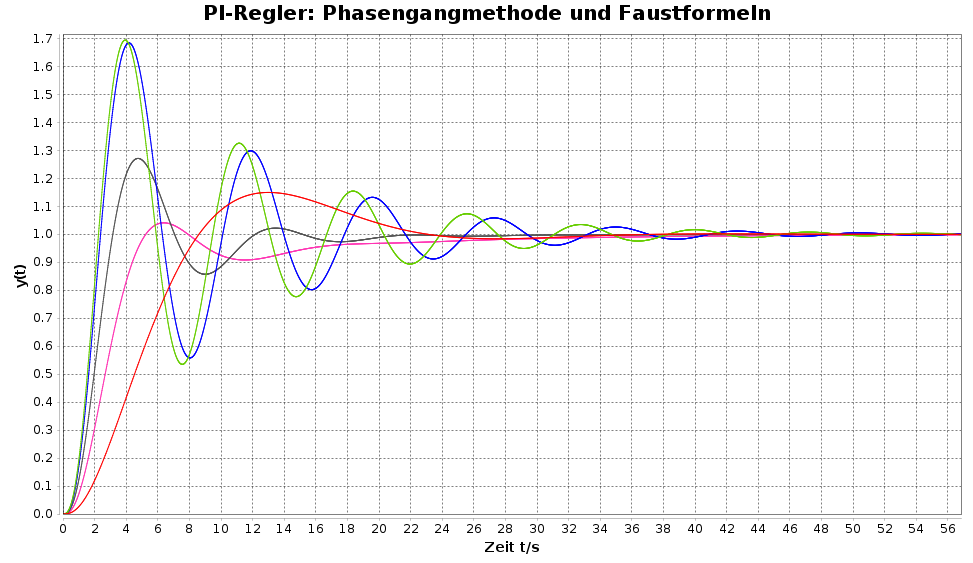
\includegraphics[width=\textwidth]{images/comparisonPI015.png}
\end{minipage}
\begin{minipage}[c][][b]{.22\textwidth}
    \captionof{figure}{%
        Schrittantworten    des   geschlossenen    Regelkreises (PI-Regler):
        \textbf{Pink}: Chiens, Hrones, Reswick (0\% \"Uberschwingen),
        \textbf{dunkelgrau}: Chiens, Hrones, Reswick (20\% \"Uberschwingen),
        \textbf{blau}: Oppelt,
        \textbf{gr\"un}: Rosenberg,
        \textbf{rot}: Phasengangmethode.
    }
    \label{fig:comparisonPI015}
\end{minipage}

\begin{minipage}[c][][b]{.75\textwidth}
    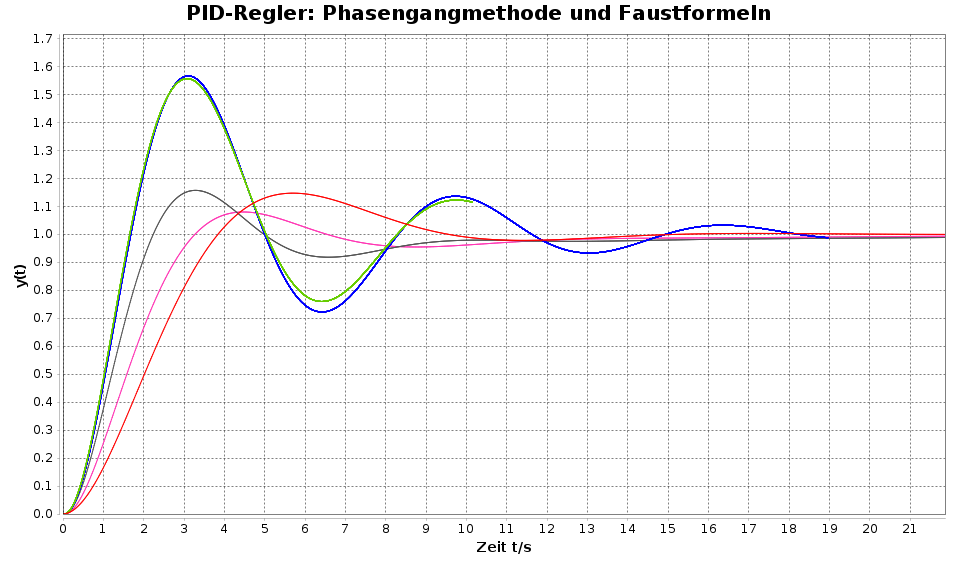
\includegraphics[width=\textwidth]{images/comparisonPID015.png}
\end{minipage}
\begin{minipage}[c][][b]{.22\textwidth}
    \captionof{figure}{%
        Schrittantworten    des   geschlossenen    Regelkreises (PID-Regler):
        \textbf{Pink}: Chiens, Hrones, Reswick (0\% \"Uberschwingen),
        \textbf{dunkelgrau}: Chiens, Hrones, Reswick (20\% \"Uberschwingen),
        \textbf{blau}: Oppelt,
        \textbf{gr\"un}: Rosenberg,
        \textbf{rot}: Phasengangmethode.
    }
    \label{fig:comparisonPID015}
\end{minipage}

\begin{minipage}[c][][b]{.75\textwidth}
    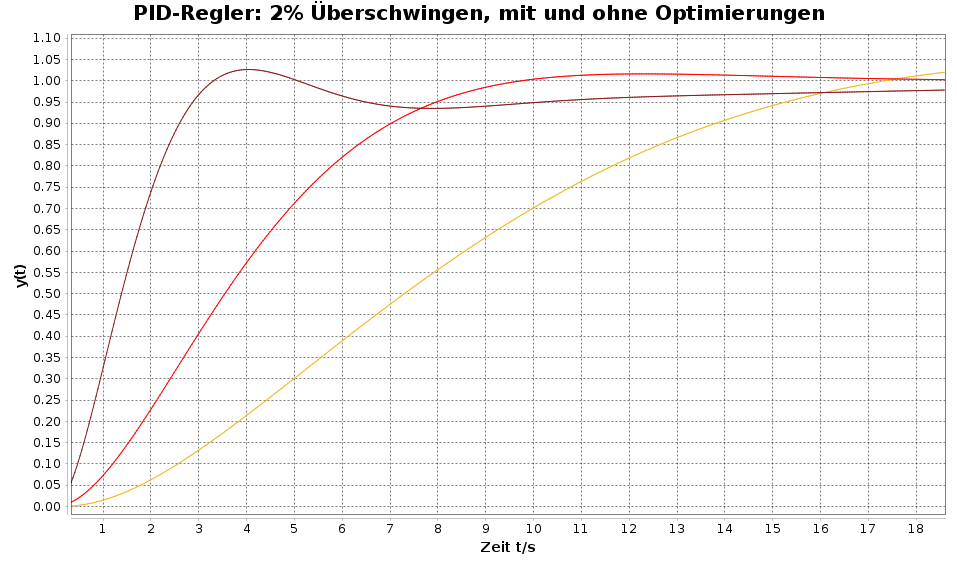
\includegraphics[width=\textwidth]{images/comparisonPID002optimisations.png}
\end{minipage}
\begin{minipage}[c][][b]{.22\textwidth}
    \captionof{figure}{%
        Schrittantworten    des   geschlossenen    Regelkreises (PID-Regler),
        \"Uberschwingen auf 2\% begrenzt, mit Optimierungen:
        \textbf{rot}: Phasengangmethode (Standardwerte),
        \textbf{braun}: Phasengangmethode (positiv optimiert),
        \textbf{gelb}: Phasengangmethode (negative optimiert).
    }
    \label{fig:comparisonPID002optimisations}
\end{minipage}


\clearpage
\subsection{Umrechnung zwischen bodekonformer und reglerkonformer Darstellung}
\label{subs:bode_regler}
Ein Regler  kann mittels verschiedener mathematischen  Gleichungen dargestellt
werden.  F\"ur  die Berechnungen  in diesem Projekt  sind zwei  von besonderer
Bedeutung: Die bodekonforme und die reglerkonforme Darstellung.

Dabei gilt  es zu  beachten, dass  sich die  einzelnen Darstellungen  in ihrer
mathematischen Gleichung  unterscheiden, jedoch den  selben Informationsinhalt
haben. Deshalb   ist  es   auch  m\"oglich,  mittels  einfacher   Umrechnungen
die  Darstellungsweise   zu  wechseln.

Der  Grund,   weshalb  zwei  verschiedene  Darstellungsarten   existieren  und
verwendet werden, liegt zum einen darin, dass gewisse Berechnungen automatisch
die eine oder andere Darstellungsart  zur\"uckgeben, jedoch auch, dass je nach
Situation der  Verst\"andlichkeit halber die eine  oder andere Darstellungsart
bevorzugt wird.

Bei der  bodekonformen Darstellung wie  in Gleichungen~\ref{eq:pi:bodekonform}
und~\ref{eq:pid:bodekonform}   ist   die  \"Ubertragungsfunktion   leicht   zu
interpretieren,  was ihren  Amplitduden- und  Frequenzgang betrifft.   Deshalb
wird  die  bodekonforme  Darstellung  \"uberall dort  verwendet,  wo  mit  den
Reglerwerten Berechnungen ausgef\"uhrt werden.

\begin{equation} \label{eq:pi:bodekonform}
    H_{rpi} = K_{rk} \cdot \biggl[ \frac{1 + s \cdot T_{nk}}{s \cdot T_{nk}} \biggr]
\end{equation}

\begin{equation} \label{eq:pid:bodekonform}
    H_{rpid} = K_{rk} \cdot \biggl[ \frac{(1 + s \cdot T_{nk}) \cdot (1 + s \cdot T_{vk}) }{ s \cdot T_{nk} } \biggr]
\end{equation}


Die reglerkonforme  Darstellung aus  den Gleichungen~\ref{eq:pi:reglerkonform}
und~\ref{eq:pid:reglerkonform}  hingegen ist  so  aufgebaut,  dass die  Werte,
welche  an  einem realen  Regler  einstellbar  sind, direkt  abgelesen  werden
k\"onnen. Diese Darstellung  wird verwendet,  um die Reglerwerte  dem Benutzer
zur Verf\"ugung zu stellen.

\begin{equation} \label{eq:pi:reglerkonform}
    H_{rpi} = K_{r} \cdot \biggl[ 1 + \frac{1}{s \cdot T_{n}} \biggr]
\end{equation}

\begin{equation} \label{eq:pid:reglerkonform}
    H_{rpid} = K_{r} \cdot \biggl[ 1 + \frac{1}{s \cdot T_n} + \frac{s \cdot T_v}{s \cdot T_p} \biggr]
\end{equation}

Zudem   liegt   das   Ergebnis   der    Faustformeln   auch   immer   in   der
reglerkonformen  Darstellung  vor. F\"ur  die  Umrechnung  zwischen  den  zwei
Darstellungsarten  ergibt  sich  durch  einen  Koeffizientenvergleich  Tabelle

\ref{tab:bode_regler_konform}.

\begin{longtable}{l|ll}
    \toprule

    %\multicolumn{3}{l}{\large{\textsc{auftragsanalyse und hintergrundinformationen}}} \\
    %\multicolumn{2}{l}{pi}

    &
    bodekonform $\rightarrow$ reglerkonform
    &
    reglerkonform $\rightarrow$ bodekonform
    \\

    \midrule

    \endhead
    \endfoot
    \endlastfoot

    % content here ---------------------------------------------------------- %

    PI
    &
    $T_n = T_{nk} $ %reglerkonform
    &
    $K_{rk} = K_r $ %bodekonform
    \\

    \midrule

    PID
    &
    $T_n = T_{nk}+T_{vk}-T_p$
    &
    $T_{nk}=0.5 \cdot (T_n+T_p) \cdot (1+\epsilon)$
    \\

    &
    $T_v=\frac{T_{nk} \cdot T_{vk}}{T_{nk}+T_{vk}-T_p}-T_p$
    &
    $T_{vk}=0.5 \cdot (T_n+t_p) \cdot (1-\epsilon)$
    \\

    &
    %$k_r=k_{rk} \cdot \frac{1+t_{vk}}{t_{nk}}$
    $K_r=K_{rk} \cdot (1 + \frac{T_{vk}-T_p}{T_{nk}})$
    &
    $K_{rk} = 0.5 \cdot K_r \cdot (1 + \frac{T_p}{T_{nk}}) \cdot (1+\epsilon )$
    \\
    \\

    &
    \multicolumn{2}{l}{wobei $\epsilon^2 = 1-(4 \cdot T_n \cdot \frac{T_v-T_p}{(T_n+T_p)^2})$}
    \\
    \bottomrule
    \caption{Formeln zur Umrechung zwischen bode- zu reglerkonformer Darstellung \cite{regelungstechnik:zellweger}, \cite{regelungstechnik:schumleon}}
    \label{tab:bode_regler_konform}
\end{longtable}


F\"ur die Berechnungen in diesem Projekt wird, wenn nicht anders angegeben, mit $T_p=\frac{1}{10} \cdot T_v$ gerechnet.


\clearpage
\subsection{Berechnung der Schrittantwort des geschlossenen Regelkreises}
\label{subs:fft}
In  diesem Projekt  ist  im speziellen  die  Schrittantwort des  geschlossenen
Regelkreises von  Bedeutung. Um auf die  Schrittantwort zu gelangen  wurde der
Weg \"uber die IFFT (Englisch:  \emph{Inverse Fast Fourier Transform}, inverse
schnelle Fourier-Transformation)  gew\"ahlt, da diese relativ  einfach in Java
zu implementieren ist.

F\"ur diese Berechnung sind folgende Schritte notwendig:

\begin{itemize}
    \item
        \"Ubertragungsfunktion des geschlossenen Regelkreises bilden
    \item
        Definition der Abstastfrequenz $f_s$ sowie der Anzahl zu berechnender Punkte
    \item
        diskreten Frequenzgang berechnen
    \item
        Frequenzgang f\"ur die IFFT vorbereiten
    \item
        Frequenzgang mittels IFFT r\"ucktransformieren
    \item
        Schrittantwort aus der Impulsantwort bilden
\end{itemize}


% --------------------------------------------------------------------------- %
\subsubsection*{\"Ubertragungsfunktion des geschlossenen Regelkreises bilden}
% --------------------------------------------------------------------------- %

Da  die \"Ubertragungsfunktionen  des Reglers  sowie der  Regelstrecke bekannt
sind,  kann aus  ihnen  die gesamte  \"Ubertragungsfunktion $H_g(s)$  gebildet
werden. Dazu  werden jeweils  die Z\"ahler-  sowie die  Nennerpolynome mittels
diskreter  Faltung  zusammengef\"uhrt. Zus\"atzlich   muss  das  resultierende
Z\"ahlerpolynom zum Nennerpolynom addiert werden.

\begin{gather} \label{eq:fft:hg}
    \begin{split}
        H_g(s)  & = \frac{ZAH(s)}{NEN(s)} \\
                & = \frac{ZAH_{Regler} \cdot ZAH_{Strecke}}{NEN_{Regler} \cdot NEN_{Strecke} + ZAH_{Regler} \cdot ZAH_{Strecke}}
    \end{split}
\end{gather}

Die Z\"ahler- und Nennerpolynome haben dabei folgende Form:

\begin{gather*}
    \begin{split}
        ZAH_{Regler}  & = b_{R_1} s^n  + b_{R_2} s^{n-1}  + \dotsb  + b_{R_{n-1}}     ~\biggr \rvert~ n \in  \mathbb{N} \\
        ZAH_{Strecke} & = b_{S_1} s^k  + b_{S_2} s^{k-1}  + \dotsb  + b_{S_{k-1}}     ~\biggr \rvert~ k \in  \mathbb{N}  \\
        NEN_{Regler}  & = a_{R_1} s^m  + a_{R_2} s^{m-1}  + \dotsb  + a_{R_{m-1}}     ~\biggr \rvert~ m \in  \mathbb{N}  \\
        NEN_{Strecke} & = a_{S_1} s^l  + a_{S_2} s^{l-1}  + \dotsb  + a_{S_{l-1}}     ~\biggr \rvert~ l \in  \mathbb{N}
    \end{split}
\end{gather*}


 --------------------------------------------------------------------------- %
\subsubsection*{Bestimmen der Abtastrate fs sowie der Anzahl zu berechnender Punkte.}
% --------------------------------------------------------------------------- %

F\"ur die Berechnung von $f_s$ durften  wir eine Methode verwenden, welche uns
von  Prof. Dr. Richard Gut  zur  Verf\"ugung  gestellt wurde. Diese  berechnet
$f_s$ anhand der Nullstellen des  Nennerpolynoms und ermittelt gleichzeitig in
Abh\"angigkeit von $f_s$  die Anzahl $N$ zu  berechnender Punkte. Deren Anzahl
ist stets  eine Potenz von  2. An dieser Stelle  wird nicht weiter  auf diesen
Schritt eingegangen; das Matlab-File  kann in Anhang~\ref{app:fftgut} gefunden
werden.


% --------------------------------------------------------------------------- %
\subsubsection*{Diskreten Frequenzgang berechnen}
% --------------------------------------------------------------------------- %

Nun  werden  f\"ur  $s$  genau $\frac{N}{2}$  Werte  eingesetzt,  welche  sich
geichm\"assig zwischen 0  und $f_s \cdot \pi$  verteilen. Dadurch entsteht ein
diskreter Frequenzgang $H_g[k]$ mit $\frac{N}{2}$ Werten.

\begin{equation}
    H_g[k] = H_g(s) ~\biggr \rvert~ s=j \cdot \frac{f_s \cdot \pi}{\frac{N}{2} - 1} \cdot k \land 0 \leq k < \frac{N}{2} \land k \in \mathbb{N}_0
\end{equation}


% --------------------------------------------------------------------------- %
\subsubsection*{Frequenzgang f\"ur die inverse Fourier-Transformation vorbereiten}
% --------------------------------------------------------------------------- %
Damit  nach  der  Transformation  in  den  Zeitbereich  ein  reelles  Resultat
vorliegt, muss der diskrete  Frequenzgang $H_g[k]$ folgende Symmetriebedingung
erf\"ullen ($L$ ist die L\"ange des Arrays $H_g$):

\begin{equation}
    H_g[L-k]=H_g^*[k]  ~\biggr \rvert~ 0 \leq k \leq L \land k \in \mathbb{N}_0
\end{equation}

Deshalb wird $H_g[\frac{N}{2}]  = 0$ gesetzt und der zweite  Teil von $H_g[k]$
jeweils durch die entsprechende Konjugiert-Komplexe $H^*[k]$ erg\"anzt.

% --------------------------------------------------------------------------- %
\subsubsection*{Frequenzgang r\"ucktransformieren}
% --------------------------------------------------------------------------- %
Die  diskrete inverse  Fourier-Transformation wird  gem\"ass folgender  Formel
durchgef\"uhrt:

\begin{equation}
    h[k]  = \frac{1}{N}  \cdot \displaystyle\sum_{n=0}^{N-1}  H[n] \cdot
    e^{j 2\pi \cdot \frac{n \cdot k}{N}} \biggr \rvert 0 \leq k < N \land k \in \mathbb{N}_0
\end{equation}

Die in diesem Projekt verwendetete inverse schnelle Fourier-Transformation ist
ein  verbessertes Verfahren  der oben  erkl\"arten IFFT.   Dieses erm\"oglicht
eine   schnellere  Berechnung   durch  das   Zerlegen  der   Punkte  in   ihre
Primfaktoren. Eine genauere Erl\"auterung wird an dieser Stelle nicht gemacht,
da  dieses  Verfahren  in  Matlab  sowie in  Java  als  lauff\"ahige  Funktion
verf\"ugbar ist.


% --------------------------------------------------------------------------- %
\subsubsection*{Schrittantwort aus der Impulsantwort bilden}
% --------------------------------------------------------------------------- %
Aus  der  Impulsantwort $h[k]$  kann  nun  in  einem einfachen  Verfahren  die
Schrittantwort  $y[k]$ gebildet  werden.  Dabei  entspricht jedes  Element der
Schrittantwort  $y[k]$ der  Summe der  Elemente der  Impulsantwort $h[k]$  vom
ersten  bis zum  k-ten Element.   Zus\"atzlich  wird die  zweite H\"alfte  der
Impulsantwort  weggeschnitten,  um  die  zuvor  als  konjugert-komplexe  Werte
hinzugef\"ugten \"Uberbleibsel zu eliminieren.

\begin{equation}
    y[k]= \sum_{n=0}^k h[n] ~\biggr \rvert~ 0 \leq k < \frac{L}{2} \land k \in \mathbb{N}_0
\end{equation}




% **************************************************************************** %
\clearpage
\section{Software}
\label{sec:software}
% **************************************************************************** %
% section Software
Leserf\"uhrung, Kontext und Top-Down  Beschreibung der Gesamtsoftware gem\"ass
Dokument Richard Gut. Verweis auf Klassendiagramm.


% ------------------------------------------------------------------------------
\subsection{View}
% ------------------------------------------------------------------------------

Leserf\"uhrung View.
Ausschnitt Klassendiagramm, Verweis auf gesamtes Diagramm.

Die  \emph{View} ist  aus  zwei \"ubergeordneten  Panels aufgebaut. Im  linken
Panel befinden sich Ein- und  Ausgabefelder f\"ur numerische Werte, das rechte
Panel  beheimtated die  Plots sowie  das Optimierungs-Panel  und kann  mittels
Check-Box "erweiter" ein- und ausgeblendet werden.

\todo{Image Gesamt-GUI}

\todo{Image Panel Schrittantwort vermessen}


Im  Bereich 1  \todo{Image Referenzen}  werden die  Parameter der  vermessenen
Strecke  eingegeben. Darunter  befinden  sich die  Schalftfl\"achen  zur  Wahl
\todo{Image Butttons  PI-, PID-T1-Regler}  zwischen der  Dimensionierung eines
PI- respektive eines PID-T1-Reglers.

Das   Panel    \emph{Reglerwerte}   dient   der   Ausgabe    der   berechneten
Reglerwerte  der   verschiedenen  Berechnungsmethoden. Ebenfalls   kann  f\"ur
die  Phasengang-Methode,   sofern  ein  PID-Regler  dimensioniert   wird,  die
Zeitkonstante  $T_p$  \todo{Check:  korrekter  Begriff}  spezifiziert  werden.
\todo{Image Panel Phasengangmethode}

Das Optimierungs-Panel  beinhaltet zwei  Slider zur Eingabe  des gew\"unschten
\"Uberschwingens   respektive   f\"ur   die  Optimierung   des   Reglers   der
Phasengang-Methode.

Unterhalb des  Optimierungs-Panels werden  die Plots der  mittels Faustformeln
und Phasengangmethode errechneten Schrittantworten graphisch ausgegeben. Diese
k\"onnen   mittels  Check-Boxen   zu-  und   weggeschaltet  werden. Zu   jeder
Faustformel wird die zugeh\"orige Schrittantwort abgebildet. Die Resultate der
Phasengangmethode  werden durch  drei Kurven  dargestellt. Eine Kurve  benutzt
den  Standardwert des  Phasenrands gem\"ass  Zellweger \todo{Einf\"ugen  Wert,
Referenz}, die beiden anderen Kurven basieren auf Benutzereingaben f\"ur einen
oberen  und  unteren  Offset  des Phasenrandes  der  \"uber  den  Schiebregler
\emph{Optimierung} eingestellt werden kann.



% ------------------------------------------------------------------------------
\subsection{Controller}
% ------------------------------------------------------------------------------

Leserf\"uhrung Controller.
Ausschnitt Klassendiagramm, Verweis auf gesamtes Diagramm.

Der  \emph{Controller}   ist  verantwortlich  f\"ur  die   Steueraufgaben  und
erzeugt    den    Regler. Da    \emph{Regler}   \"ubersetzt    auf    Englisch
\emph{Controller} ist, heisst die  generische Reglerklasse in unserer Software
\emph{Controller}. Die  Klasse, welche  die  die  Rolle des  \emph{Controller}
im   Kontext   von   \emph{Model-View-Controller}  wahrnimmt,   heisst   daher
\emph{GUIController}, um Namenskonflikte zu vermeiden.



% ------------------------------------------------------------------------------
\subsection{Model}
% ------------------------------------------------------------------------------

Leserf\"uhrung Controller.
Ausschnitt Klassendiagramm, Verweis auf gesamtes Diagramm.

Im Model wird f\"ur jede Berechnungsart, also entwerder f\"ur die Faustformeln
oder die Phasengangmethode, Objekt des Typs \code{CloseLoop} erzeugt.


\subsubsection*{Controller}

Der  Controller  bildet  die  Oberklasse   f\"ur  alle  Faustformeln  und  die
Phasengangmehode. Sie  beinhaltet  die  abstrakte  Methode  \code{calculate()}
sowie alle n\"otigen Getter und Setter.


\subsubsection*{Faustformeln}

\code{Chien20},   \code{ChienApper},   \code{Oppelt},   \code{Rosenberg}   und
\code{ZieglerNichols} sind die Klassen  zu den zugeh\"origen Fausformeln.  Die
abstrakte Methode  \code{calculate()} aus der Klasee  \code{Controller} ist in
jeder dieser Klassen  implementiert. Sie liest die ben\"otigten  Werte aus der
Strecke (Klasse  \code{Path}) aus  und f\"uhrt  die Berechnungen  gem\"ass der
entsprechenden Faustformel aus.


\subsubsection*{ClosedLoop}

In  der  Klasee  \code{ClosedLoop}   wird  f\"ur  jede  Berechungsart  jeweils
ein  \code{Controller}  erstellt. Auch  diese Klasse  enth\"alt  eine  Methode
\code{calculate()}. In   dieser  wird   einerseits   f\"ur  alle   Rechenarten
die  Berechung   der  Schrittantwort   mittels  \code{calculateStepResponse()}
ausgel\"ost   und   f\"ur   die  Phasengangmethode   wird   zus\"atzlich   das
\"Uberschwingverhalten durch \code{overShootOptimazation()} optimiert.


\subsubsection*{PhaseRespsonseMethod}

\todo{Dieser  Abschnitt  sollte  vermutlich nomals  Aufmerksamkeit  von  einem
Experten zum Code erhalten.}

In dieser Klasse  wird die Frequenzachse in Abh\"angigkeit  vom Phasengang und
des ben\"otigten Winkelbereiches erstellt.   Ausserdem finden wir verschiedene
calculate Methoden.

Einerseits  ist da  calculate()  , in  dieser  wird die  UTF  Strecke aus  der
Strecke(path)  geholt  und  die  Omega-Achse  Methode  aufgeruffen. In  dieser
wird Sie  Abh\"angigkeit vom  Phasengang und des  ben\"otigten Winkelbereiches
erstellt.

Anschlissend werden die Werte f\"ur Hs und phiS berehnet.

Andererseits  sind  da die  Methoden,  calculateTnvTnk()  um  Tnk und  Tnv  zu
berechnen, calculateKrk um Krk zu berechnen, calculatecontrollerConf() um eine
umrechung  von Bodekonformen  Werten  zu Reglerkonformen  Werten  in der  calc
Klasse  auszul\"osen, calculatePhaseMargin()  bestimmt je  nach Reglertyp  den
Phasenrand  und zum  schluss calculateOverShoot(),  hier wird  je nach  vorher
berechnetem \"Uberschwingen, dem  Wert phiu einen der  4 vordefinierten static
final Werte zugewiesen.



% ------------------------------------------------------------------------------
\subsection{Benutzungs-Beispiel (Use-Case)}
% ------------------------------------------------------------------------------

Leserf\"uhrung Use-Case.
Ausschnitt Klassendiagramm, Verweis auf gesamtes Diagramm.

Das Zusammenspiel der einzelnen Komponenten  der Applikation wird im Folgenden
anhand  eines   Beispiels  erkl\"art. Die  hier   dargelegten  Zusammenh\"ange
k\"onnen   auch   gut   im   Klassendiagramm   (Anhang~\ref{app:classdiagram})
betrachtet werden.

Beim   Programmstart   werden   durch  das   Model   drei   \code{closedLoops}
(geschlossener  Regelkreis) f\"ur  die Phasengangmethode  sowie vier  weitere
f\"ur  die Faustformeln  erzeugt. Jeder \code{closedLoops}  ist von  Beginn an
einem  Berechnungstyp  (Phasengangmethode,  Faustformel)  zugewiesen. Er  ist
bereit, Daten aufzunehmen und zu verarbeiten.

\"Uber die  drei Eingabefelder  $K_s$, $T_u$  und $T_g$  werden die  Werte der
vermessenen Regelstrecke  durch den  Benutzer eingegeben. Durch  Dr\"ucken des
Buttons  „Berechnen“ werden  die Eingaben  durch den  \code{GUIController} auf
Zul\"assigkeit  \"uberpr\"uft. Erf\"ullen  sie  die  erforderlichen  Kriterien
nicht,  wird eine  Benachrichtigung mit  Hinweis auf  den Fehler  oberhalb des
Buttons ausgegeben und die Berechnung nicht ausgel\"ost.

Haben  die   Eingaben  die  \"Uberpr\"ufung  durch   den  \code{GUIController}
bestanden,  fragt  dieser  zus\"atzlich  die  aktuellen  Werte/Zust\"ande  der
Slider  f\"ur \"Uberschwingen  und  Optimierung sowie  den  Reglertyp auf  dem
GUI  ab  und   leitet  alle  Daten  mittels  \code{setData()}   an  das  Model
weiter. Dieses erzeugt  einen Path (Strecke) aus  den Eingabewerten. Das Model
errechnet  den  Optimierungs-Offset und  weist  die  Daten den  entsprechenden
\code{closedLoops} der  Phasengangmethode sowie der Faustformeln  mittels der
Methode \code{setData()}  zu. Jeder \code{ClosedLoop} leitet die  Daten an den
zugeh\"origen  Controller weiter,  der  die  Reglerwerte berechnet. Zu  Beginn
betrachten wir den Regler nach Oppelt genauer.

Die  Klasse \code{Oppelt}  erbt  von der  abstrakten Klasse  \code{Controller}
und  besitzt  somit  alle  Setter-  und  Getter-Methoden  der  Oberklasse. Als
Input  stehen die  Informationen der  Strecke  sowie der  Reglertyp (PI,  PID)
zur  Verf\"ugung. Je nach  gew\"ahltem Berechnungstyp  werden die  Reglerwerte
reglerkonform  berechnet  und  gespeichert. Weiter  werden die  Werte  in  die
bodekonforme  Darstellung umgerechnet  und  ebenfalls  abgespeichert (mehr  zu
diesem Thema in Abschnitt~\ref{subs:bode_regler}).

Die    Berechnungstypen   Rosenberg,    Chien/Hrones/Reswick   (20\%)    sowie
Chien/Hrones/Reswick (aperiod.) funktionieren analog dem Berechnungstyp Oppelt
und werden nicht weiter ausgef\"uhrt.

Ein   spezielles  Augenmerk   richten   wir  nun   auf   die  Berechnung   der
Phasengangmethode. Auch  die   Klasse  \code{PhaseResponseMethod}   erbt  von
der  Klasse  \code{Controller}  und  bringt die  bereits  erw\"ahnten  Setter-
und   Getter-Methoden  mit. Die   Input-Werte  sind   analog  derjenigen   der
Faustformeln. Zus\"atzlich  werden  die   Informationen  zum  \"Uberschwingen,
der   Optimierung   sowie   $T_p$   in  die   Berechnung   miteinbezogen   und
die   gesetzten  Input-Werte   werden  den   lokalen  Attributen   zugewiesen.
\code{calculateOvershoot()}   wird   ausgel\"ost   und  setzt   das   Attribut
\code{phiU},   welches   f\"ur   das   korrekte   \"Uberschwingen   ben\"otigt
wird. Darauf   folgend  wird   \code{calculate()}  aufgerufen. Diese   Methode
berechnet   anhand   der   Methode   \code{createOmegaAxis()}   die   diskrete
Omega-Achse  in  Abh\"angigkeit  der  Zeitkonstanten  der  Regelstrecke.   Der
Wert  der  \"Ubertragungsfunktion  der  Regelstrecke wird  f\"ur  alle  Punkte
der Frequenzachse  ausgewertet. \code{calculateTnk()}  wird ausgel\"ost. Diese
Methode  berechnet   $T_nk$  und  $T_vk$  unter   Zuhilfenahme  der  diskreten
Werte   nach  dem   Prinzip  der   Phasengangmethode. Daraus  resultiert   die
\"Ubertragungsfunktion  des   Reglers. Falls  $T_p   =  0$  aus   der  Eingabe
\"ubergeben   wurde,  wird   an  dieser   Stelle  $T_p   =  \frac{T_{vk}}{10}$
gesetzt. $K_{rk}$    wird     gem\"ass    der     Phasengangmethode    mittels
\code{calculateKrk()}     berechnet. Zudem      beinhaltet     die     Methode
\code{calculateKrk()}   den    Aufruf   von   \code{calculateControllerConf()}
und   \code{setUTF()}.   \code{calculateControllerConf()}  transformiert   die
Werte   in  die   reglerkonforme   Darstellung.   \code{setUTF()}  setzt   die
\"Ubertragungs-Funktion des Reglers.

Im    \code{ClosedLoop}    wird    nun    die    Methode    \code{calculate()}
ausgef\"uhrt,  welche   mittels  der   Methode  \code{calculateStepResponse()}
die   Schrittanwort  des   geschlossenen   Regelkreises  berechnet. Falls   es
sich  bei  der  Berechnungsmethode   des  Reglers  um  die  Phasengangmethode
handelt,  wird  zus\"atzlich \code{overShootOptimization()}  (dokumentiert  in
Anhang~\ref{app:algo:oversh}) aufgerufen. Diese Methode  \"andert den Wert von
$K_{rk}$ so lange, bis das gew\"unschte \"Uberschwingen erreicht wird.

Sobald die  Berechnungen aller \code{ClosedLoops} abgeschlossen  sind, wird im
\code{Model}  die  Methode \code{notifyObserver()}  ausgel\"ost. Hiermit  wird
die  \code{View}  dar\"uber  informiert,  dass  \"Anderungen  im  \code{Model}
vorgenommen  wurden   und  die  Methode  \code{update()}   in  den  jeweiligen
Unterklassen der Klasse  \code{View}aufgerufen werden soll. Somit aktualisiert
sich die \code{View} und  die neu berechneten Reglerwerte. Die Streckenordnung
wird  ausgegeben   und  die   Plot-Daten  werden  aktualisiert. Im   Fall  der
Phasengangmethode werden auch Startwerte f\"ur $T_p$ gesetzt.

Der Benutzer  hat nun die  M\"oglichkeit, die Resultate  der Phasengangmethode
weiter  zu  optimieren. \"Uber  das   Panel  \code{Optimierungen}  stehen  die
Slider  \emph{\"Uberschwingen} sowie  \emph{Optimierung} zur  Verf\"ugung. Das
\"Uberschwingen  kann  in  vorgegebenen   Schritten  in  Prozenten  festgelegt
werden. Die  Optimierung  schiebt  $\varphi_{start}$  in  die  positive  sowie
negative   Richtung   zugleich  und   wird   mittels   zwei  separaten   Plots
dargestellt. Weiter k\"onnen  die Werte f\"ur $T_p$  nachtr\"aglich f\"ur jede
der drei Kurven individuell angepasst werden.

Sobald  einer   der  drei  Parameter  (\"Uberschwingen,   Optimierung,  $T_p$)
ver\"andert  wird,   wird  \"uber   den  \code{GUIController}   die  jeweilige
Setter-Methode im \code{Model} aufgerufen. Das  \code{Model} gibt die Daten an
den jeweiligen \code{ClosedLoop}  weiter, der diese wiederum  den Methoden der
Phasengangmethode  weiterleitet. Sobald die  neu berechneten  Werte vorliegen
wird \code{notifyObservers()} aufgerufen und die \code{View} aktualisiert.

Die  Plots  sowie die  Optimierungs-Schaltfl\"achen  sind  nur dann  sichtbar,
wenn die  CheckBox \emph{erweitert}  aktiviert ist. Durch  Deaktivieren dieser
CheckBox  kann das  Programm  in einer  Klein-Ansicht  ohne grafische  Ausgabe
bedient werden. Die  einzelnen Plots k\"onnen \"uber  CheckBoxen unterhalb des
Plot-Bereichs dazu- oder weggeschaltet werden.

\"Uber  den Button  \emph{L\"oschen}  k\"onnen alle  Regler- sowie  Plot-Daten
gel\"oscht werden.




% **************************************************************************** %
\clearpage
\section{Verifikation}
\label{sec:test}
% **************************************************************************** %
Damit  die Software  von  Anfang an  den Anforderungen  des  Kunden sowie  dem
Pflichtenheft entspricht, wurden die Berechnungen sowie die Funktionsweise der
einzelnen Komponenten laufend mittels verschiedenster Varianten \"uberpr\"uft,
welche nachfolgend erl\"autert werden.

\subsection{Berechnungen}
Die  Berechnungen und  Algorithmen wurden  vorerst in  Matlab geschrieben  und
durch  ein  weiteres  Teammitglied \"uberpr\"uft. Die  in  Matlab  berechneten
Test-Resultate konnten mit  dem Fachcoach/Auftraggeber abgeglichen werden. Die
so entstandenen Matlab-Files  dienten als direkte Vorlage  f\"ur die Umsetzung
in Java-Code. Zus\"atzlich  konnten die berechneten  Werte in Java  direkt mit
den Resultaten aus Matlab verglichen werden.

\subsection{Intern (Team)}
Um  die  Funktionalit\"at   und  das  Verhalten  des  GUIs   zu  testen  wurde
das  Programm  regelm\"assig  durch   das  Team  getestet. Dabei  wurden  alle
Mitglieder dazu  aufgefordert nebst den  zu erwartenden Werten  auch explizite
Fehleingaben/-ausgaben zu provozieren.

Fehler     wurden     umgehend     an     den     Programmier-Verantwortlichen
weitergeleitet. Sobald  der Fehler  behoben  wurde, wurde  das Team  dar\"uber
informiert und zur erneuten Verifikation aufgefordert.

\subsection{Extern}
Das Tool wurde auf Computer  aussenstehender Personen auf Funktionalit\"at und
korrekte  Darstellungsweise  getestet. Dabei  wurde ein  spezielles  Augenmerk
darauf  gelegt, dass  die  Testpersonen  unterschiedliche Betriebssysteme  und
Bildschirmaufl\"osungen verwenden.


\subsection{Auftraggeber}
Die Software wurde in enger Zusammenarbeit mit dem Auftraggeber entwickelt. So
konnte  er  die  Software  immer   wieder  testen  und  direktes  Feedback  an
die  Entwickler   geben. Eine  m\"oglichst  kundenorientierte   L\"osung,  die
den  Vorstellungen  des  Auftraggebers  entspricht,  konnte  somit  erarbeitet
werden. Eine  Vorabversion  wurde  dem Auftraggeber  zur  \"Uberpr\"ufung  der
Aufl\"osung und Lauff\"ahigkeit auf seinem System zugestellt.



% **************************************************************************** %
\clearpage
\section{Schlussfolgerungen}
\label{sec:schlussfolgerungen}
% **************************************************************************** %
% was laeuft, was laeuft nicht, was kann verbessert werden



% **************************************************************************** %
\clearpage
\section*{Ehrlichkeitserkl\"arung}
\label{sec:ehrlickeitserklaerung}
% **************************************************************************** %
Mit der  Unterschrift best\"atigt der Unterzeichnende  (Projektleiterin), dass
das Dokument selbst geschrieben worden ist und alle Quellen sauber und korrekt
deklariert worden sind.

\vspace*{3em}

Anita Rosenberger:  \underline{\hspace{8cm}}

\vspace*{3em}

Ort, Datum:  \underline{\hspace{5cm}},  \underline{\hspace{4cm}}



% **************************************************************************** %
\clearpage
%\phantomsection
\appendix
\addcontentsline{toc}{section}{Appendix}
% **************************************************************************** %
\clearpage
% ------------------------------------------------------------------------------
\section{Manuelle Berechnung des Hilfsparameteres $\beta$}
% ------------------------------------------------------------------------------
\label{app:beta}
Der   erste  Iterationsschtitt   der  in   Abschnitt~\ref{subs:phasengang:pid}
erw\"ahnten  manuellen Berechnung  des  Hilfsparameteres $\beta$  ist hier  im
Detail ausgef\"uhrt.

Zur  Rekapitulation   eine  kurze   Wiederholung  der   Ausgangslage:

\begin{gather} \label{eq:app:recap}
    \begin{split}
        \omega_{pid} & = \SI{0.6714}{\per\second} \\
        {T_{vk}}     & = \frac{\beta}{\omega_{pid}}  = \frac{0.5}{\SI{0.6714}{\per\second}}                   = \SI{0.7447}{\second} \\
        {T_{nk}}     & = \frac{1}{\omega_{pid} \cdot \beta} = \frac{1}{\SI{0.6714}{\per\second} \cdot 0.5 }  = \SI{2.9789}{\second}  \\
        K_{rk}       & = 1
    \end{split}
\end{gather}

Diese Werte eingesetzt in Gleichung~\ref{eq:pid:target} ergeben:

\begin{gather} \label{eq:app:h_rpid:start}
    \begin{split}
        H_{rpid}(j\omega)
                 & = K_{rk} \cdot \biggl[ \frac{(1 + s       \cdot T_{nk}              ) (1 + s       \cdot T_{vk}              )}{ s       \cdot T_{nk} }              \biggr] \\
                 & =      1 \cdot \biggl[ \frac{(1 + j\omega \cdot \SI{0.7447}{\second}) (1 + j\omega \cdot \SI{2.9789}{\second})}{ j\omega \cdot \SI{2.9789}{\second}} \biggr] \\
                 & = \frac{%
                                1
                                +
                                j\omega
                                \cdot (
                                          \SI{2.9789}{\second}
                                          +
                                          \SI{0.7447}{\second}
                                      )
                                -
                                \omega^2
                                \cdot
                                \SI{0.7447}{\second}
                                \cdot
                                \SI{2.9789}{\second}
                           }{%
                                j\omega
                                \cdot
                                \SI{2.9789}{\second}
                           } \\
                 & = \frac{1 - \SI{2.2184}{\square\second} \cdot \omega^2 + j\omega \cdot \SI{3.7236}{\second}}{j\omega \cdot \SI{2.9789}{\second}} \\
                 & = \frac{-\omega \cdot \SI{3.7236}{\second} + j (1 - \omega^2 \cdot \SI{2.2184}{\square\second})}{\omega \cdot \SI{2.9789}{\second}} \\
                 & = -1.250 + j \cdot (\omega^{-1} \cdot \SI{0.3357}{\per\second} - \omega \cdot \SI{0.7450}{\second})
    \end{split}
\end{gather}

Von   dieser   Zahl   gilt   es   nun,   das   Argument   zu   bestimmen   und
abzuleiten. $H_{rpid}(j\omega)$ ist eine komplexe Zahl in der linken Halbebene
($Re <  0$), somit  kommen folgende  Formeln zur  Berechnung des  Arguments in
Frage:

\begin{gather} \label{eq:app:argument}
    \begin{split}
        \varphi(Re + j \cdot Im) = atan \biggl( \frac{Im}{Re} \biggr) + \pi \hspace{2em} Re < 0 \land Im \geq 0 \\
        \varphi(Re + j \cdot Im) = atan \biggl( \frac{Im}{Re} \biggr) - \pi \hspace{2em} Re < 0 \land Im < 0
    \end{split}
\end{gather}

Da aber in diesem Fall lediglich die \emph{Ableitung} von $\varphi$ ben\"otigt
wird, f\"allt der Summand $\pm\pi$ weg  und welche Formel f\"ur die Berechnung
des  Arguments   verwendet  wird,  ist  ohne   Konsequenz.

\begin{gather} \label{eq:app:argument_numerical}
    \begin{split}
        \varphi(H_{rpid}(j\omega)) & = atan \biggl( \frac{ \omega^{-1} \cdot \SI{0.3357}{\per\second} - \omega \cdot \SI{0.7450}{\second} }{ -1.250 } \biggr) \pm \pi \\
                                   & = atan \biggl( \omega^{-1} \cdot \SI{-0.2686}{\per\second}       - \omega \cdot \SI{0.5960}{\second}             \biggr) \pm \pi
    \end{split}
\end{gather}

Die Ableitung des Arkustangens ist:

\begin{equation} \label{eq:app:d_atan}
    \frac{d}{dx} atan(x) = \frac{1}{1+x^2}
\end{equation}

Mit

\begin{equation} \label{eq:app:x_of_omega}
    x(j\omega) = \omega^{-1} \cdot \SI{-0.2686}{\per\second} - \omega \cdot \SI{0.5960}{\second}
\end{equation}

folgt

\begin{gather} \label{eq:app:d_argument}
    \begin{split}
        \frac{d}{d\omega} \varphi(H_{rpid}(j\omega)) & = \frac{d}{dx} atan(x(j\omega)) \cdot \frac{d}{d\omega} x(j\omega) \\
                                                     & = \frac{0.5960 + \omega^{-2} \cdot \SI{0.2686}{\square\second}}{1+(\omega \cdot \SI{0.5960}{\second} - \omega^{-1} \cdot \SI{0.2686}{\per\second})^2} \\
                                                     & \approx 1.1920
    \end{split}
\end{gather}


Wie    in  Gleichung~\ref{eq:pid:phi_sum_result_iteration_one}  gezeigt,   ist
dies  noch  nicht  der  gesuchte  Wert  f\"ur  $\beta$. F\"ur  den  n\"achsten
Iterationsschritt    w\"urde     nun    ein    kleinerer     Wert    gew\"ahlt
(z.B.   $\beta=0.25$),    der   zu    neuen   Werten   f\"ur    $T_{nk}$   und
$T_{vk}$   f\"uhren   w\"urde,   mit   denen   dann   die   Berechnungen   aus
Gleichungen~\ref{eq:app:h_rpid:start}    bis~\ref{eq:app:d_argument}    erneut
ausgef\"uhrt w\"urden. Bei zufriedenstellender N\"ahe der Steigung des offenen
Regelkreises zu $-\frac{1}{2}$ ist die Iteration beendet.


\clearpage
% ------------------------------------------------------------------------------
\section{Beschreibung der Algorithmen}
% ------------------------------------------------------------------------------
\label{app:algos}
% ---------------------------------------------------------------------------- %
\subsection{Sani}
% ---------------------------------------------------------------------------- %

\subsubsection*{Input}

\begin{tabular}{p{40mm}l}
    $ T_u $ & Verzugszeit \\
    $ T_g $ & Anstiegszeit
\end{tabular}

\subsubsection*{Output}
\begin{tabular}{p{40mm}l}
    $ n $ & Ordnung der Regelstrecke \\
    $ T $ & Zeitkonstante
\end{tabular}

\subsubsection*{Algorithmus}
\begin{enumerate}
    \item
        Ung\"ultige Eingaben warden abgefangen und ein Fehler zur\"uckgegeben.
    \item
        L\"adt Werte f\"ur Tu und Tg.
    \item
        Erstellt 50 Werte zwischen 0 und 1 f\"ur ri.
    \item
        Bestimmt die Ordnung der Regelstrecke.
    \item
        Spline f\"ur r und w
    \item
        T(n) wird aus w*tg berechnet.
    \item
        Umspeichern \& Sortieren
\end{enumerate}

\subsubsection*{Matlab-Code}
\lstinputlisting[style=Matlab-editor-2]{mfiles/p2Sani.m}


\clearpage
% ---------------------------------------------------------------------------- %
\subsection{Umrechnung von reglerkonformer in bodekonforme Darstellung}
% ---------------------------------------------------------------------------- %

\subsubsection*{Input}
\begin{tabular}{p{40mm}l}
    $ T_v $        & Vorhaltezeit \\
    $ T_n $        & Nachstellzeit \\
    $ T_p $        & Periodendauer \\
    $ K_r $        & Verst\"arkungsfaktor des Reglers \\
      Reglertyp    & Typ des Reglers (P, PI, PID)
\end{tabular}

\subsubsection*{Output}
\begin{tabular}{p{40mm}l}
    $ T_{nk} $ & Nachstellzeit \\
    $ T_{vk} $ & Vorhaltezeit \\
    $ K_{rk} $ & Verst\"arkungsfaktor des Reglers
\end{tabular}

\subsubsection*{Algorithmus}
\begin{enumerate}
    \item
        W\"ahlt je nach Reglertyp die Umrechnungsformel.
    \item
        Falls der I-Regler gew\"ahlt wird, gibt der Algorithmus einen Fehler zur\"uck, da der I-Regler nicht implementiert ist.
    \item
        PI-Regler:
        $T_{nk} = T_n$, $K_{rk} = K_r$, $T_{vk} = 0$
    \item
        F\"ur PID-Regler:
        \begin{equation*}
            \varepsilon =\frac{\sqrt{1-(4 \cdot T_n \cdot (T_v-T_p))}}{(T_n+T_p)^2}
        \end{equation*}

        \begin{equation*}
            T_{nk} = \frac{(T_n+T_p) \cdot (1+\varepsilon)}{2}
        \end{equation*}

        \begin{equation*}
            K_{rk} = \frac{K_r \cdot (\frac{1+T_p}{T_{nk}}) \cdot (1+\varepsilon)}{2}
        \end{equation*}

        \begin{equation*}
            T_{vk} = \frac{(T_n+T_p)*(1+\varepsilon)}{2}
        \end{equation*}
\end{enumerate}
\subsubsection*{Matlab-Code}
\lstinputlisting[style=Matlab-editor-2]{mfiles/p2Bodekonf.m}


% ---------------------------------------------------------------------------- %
\subsection{Umrechnung von bodekonformer in reglerkonforme Darstellung}
% ---------------------------------------------------------------------------- %

\subsubsection*{Input}

\begin{tabular}{p{40mm}l}
    $ T_p  $ & Periodendauer \\
    $ T{nk} $ & Nachstellzeit \\
    $ T{vk} $ & Vorhaltezeit \\
    $ K{rk} $ & Verst\"arkungsfaktor des Reglers \\
      Reglertyp   & Reglertyp (P, PI, PID)
\end{tabular}

\subsubsection*{Output}
\begin{tabular}{p{40mm}l}
    $ T_n $ & Nachstellzeit \\
    $ T_v $ & Vorhaltezeit \\
    $ K_r $ & Verst\"arkungsfaktor des Reglers
\end{tabular}

\subsubsection*{Algorithmus}
\begin{enumerate}
    \item
        W\"ahlt je nach Reglertyp die Umrechnungsformel.
    \item
        Falls der I-Regler gew\"ahlt wird, gibt der Algorithmus einen Fehler zur\"uck, da der I-Regler nicht implementiert ist.
    \item
        PI-Regler:
        $T_{n} = T_{nk}$, $K_{k} = K_{rk}$, $T_{v} = 0$
    \item
       F\"ur PID-Regler:

       \begin{equation*}
           K_r= K_{rk} \cdot \frac{1+T_{vk}}{T_{nk}}
       \end{equation*}

       \begin{equation*}
           T_n= T_{nk}+T_{vk}-T_p
       \end{equation*}

       \begin{equation*}
           T_v = \frac{T_{nk} \cdot T_{vk}}{T_{nk}+T_{vk}-T_p)-T_p}
       \end{equation*}

\end{enumerate}

\subsubsection*{Matlab-Code}
\lstinputlisting[style=Matlab-editor-2]{mfiles/p2Reglerkonf.m}


\clearpage
% ---------------------------------------------------------------------------- %
\subsection{utfController}
% ---------------------------------------------------------------------------- %

\subsubsection*{Input}

\begin{tabular}{p{40mm}l}
    $ T_p $        & Verzugszeit \\
    $ T_{nk} $     & Nachstellzeit \\
    $ T_{vk} $     & Vorhaltezeit \\
    $ K_{rk} $     & Verst\"arkungsfaktor des Reglers \\
      Reglertyp    & Reglertyp (P, PI, PID)
\end{tabular}

\subsubsection*{Output}
\begin{tabular}{p{40mm}l}
    Z\"ahler & Reeller Z\"ahler \\
    Nenner   & Reeller Nenner
\end{tabular}\todo{korrekt? Oder einfach reelle Koeffizienten?}

\subsubsection*{Algorithmus}
\begin{enumerate}
    \item
        W\"ahlt je nach Reglertyp die korrekten Formeln.
    \item
        \todo{Matrix}
\end{enumerate}

\subsubsection*{Matlab-Code}
\lstinputlisting[style=Matlab-editor-2]{mfiles/p2UTFRegler.m}

\subsection{Faustformel Oppelt}

\subsubsection*{Input}

\begin{tabular}{p{40mm}l}
    $ T_p $        & Verzugszeit \\
    $ T_u $        & Anstiegszeit \\
    $ K_s $        & Verst\"arkung der Strecke \\
      Reglertyp    & Reglertyp (P, PI, PID)
\end{tabular}

\subsubsection*{Output}
\begin{tabular}{p{40mm}l}
    $ K_p $ & Proportionalit\"atsfaktor \\
    $ T_n $ & Nachstellzeit \\
    $ T_v $ & Vorhaltezeit
\end{tabular}

\subsubsection*{Algorithmus}
\begin{enumerate}
    \item
        W\"ahlt je nach Reglertyp die korrekten Formeln.
    \item
        F\"ur PI:
        \begin{equation*}
             K_p= \frac{0.8}{K_s} \cdot \frac{T_g}{T_u}
        \end{equation*}

        \begin{equation*}
             T_n=3 \cdot T_u
        \end{equation*}

        \begin{equation*}
              t_v=0
        \end{equation*}
    \item
        F\"ur PID:
        \begin{equation*}
            K_p = \frac{1.2}{K_s} \cdot \frac{T_g}{T_u}
        \end{equation*}

        \begin{equation*}
            T_n=2 \cdot T_u
        \end{equation*}

        \begin{equation*}
            T_v=0.42*T_u
        \end{equation*}
\end{enumerate}

\subsubsection*{Matlab-Code}
\lstinputlisting[style=Matlab-editor-2]{mfiles/p2Ffoppelt.m}


\clearpage
% ---------------------------------------------------------------------------- %
\subsection{Faustformel Rosenberg}
% ---------------------------------------------------------------------------- %

\subsubsection*{Input}

\begin{tabular}{p{40mm}l}
    $ T_p $        & Verzugszeit \\
    $ T_u $        & Anstiegszeit \\
    $ K_s $        & Verst\"arkung der Strecke \\
      Reglertyp    & Reglertyp (P, PI, PID)
\end{tabular}

\subsubsection*{Output}
\begin{tabular}{p{40mm}l}
    $ K_p $ & Proportionalit\"atsfaktor \\
    $ T_n $ & Nachstellzeit \\
    $ T_v $ & Vorhaltezeit
\end{tabular}

\subsubsection*{Algorithmus}
\begin{enumerate}
    \item
        W\"ahlt je nach Reglertyp die korrekten Formeln.
    \item
    \item
        F\"ur PI:

        \begin{equation*}
            K_p= \frac{0.91}{K_s} \cdot \frac{T_g}{T_u}
        \end{equation*}

        \begin{equation*}
            T_n=3.3 \cdot T_u
        \end{equation*}

        \begin{equation*}
            T_v=0
        \end{equation*}
    \item
        F\"ur PID:

        \begin{equation*}
            Kp = \frac{1.2}{K_s} \cdot \frac{T_g}{T_u}
        \end{equation*}  \\

        \begin{equation*}
            T_n=2 \cdot T_u
        \end{equation*}

        \begin{equation*}
            T_v=0.45 \cdot T_u;
        \end{equation*}
\end{enumerate}

\subsubsection*{Matlab-Code}
\lstinputlisting[style=Matlab-editor-2]{mfiles/p2Ffrosenberg.m}


\clearpage
% ---------------------------------------------------------------------------- %
\subsection{Faustformel Ziegler}
% ---------------------------------------------------------------------------- %

\subsubsection*{Input}

\begin{tabular}{p{40mm}l}
    $ T_p $        & Verzugszeit \\
    $ T_u $        & Anstiegszeit \\
    $ K_s $        & Verst\"arkung der Strecke \\
      Reglertyp   & Reglertyp (P, PI, PID)
\end{tabular}

\subsubsection*{Output}
\begin{tabular}{p{40mm}l}
    $ K_p $ & Proportionalit\"atsfaktor \\
    $ T_n $ & Nachstellzeit \\
    $ T_v $ & Vorhaltezeit
\end{tabular}

\subsubsection*{Algorithmus}
\begin{enumerate}
    \item
        W\"ahlt je nach Reglertyp die korrekten Formeln.
    \item
        F\"ur PI:
        \begin{equation*}
            K_p= \frac{0.9}{K_s} \cdot \frac{T_g}{T_u}
        \end{equation*}

        \begin{equation*}
            T_n=3.33 \cdot T_u
        \end{equation*}

        \begin{equation*}
            T_v=0
        \end{equation*}
    \item
        F\"ur PID:
        \begin{equation*}
            K_p = \frac{1.2}{K_s} \cdot \frac{T_g}{T_u}
        \end{equation*}

        \begin{equation*}
            T_n=2 \cdot T_u
        \end{equation*}

        \begin{equation*}
            T_v = 0.5 \cdot T_u
        \end{equation*}
\end{enumerate}

\subsubsection*{Matlab-Code}
\lstinputlisting[style=Matlab-editor-2]{mfiles/p2Ffziegler.m}

\clearpage
% ---------------------------------------------------------------------------- %
\subsection{Faustformel Chien}
% ---------------------------------------------------------------------------- %

\subsubsection*{Input}

\begin{tabular}{p{40mm}l}
    $ T_p $             & Verzugszeit \\
    $ T_u $             & Anstiegszeit \\
    $ K_s $             & Verst\"arkung der Strecke \\
      Reglertyp         & Reglertyp (P, PI, PID) \\
    \"Uberschwingen     & Flag f\"ur \"Uberschwingeng %\TODO{specifics $
\end{tabular}

\subsubsection*{Output}
\begin{tabular}{p{40mm}l}
    $ K_p $ & Proportionalit\"atsfaktor \\
    $ T_n $ & Nachstellzeit \\
    $ T_v $ & Vorhaltezeit
\end{tabular}

\subsubsection*{Algorithmus}
\begin{enumerate}
    \item
        W\"ahlt je nach Reglertyp die korrekten Formeln.
    \item
        F\"ur PI, ohne \"Uberschwingen:
        \begin{equation*}
            K_p= \frac{0.35 \cdot T_g}{K_s \cdot T_u}
        \end{equation*}

        \begin{equation*}
            T_n=1.2 \cdot T_u
        \end{equation*}

        \begin{equation*}
            T_v=0
        \end{equation*}

    \item
        F\"ur PI, 20\% \"Uberschwingen:

        \begin{equation*}
            K_p= \frac{0.7 \cdot T_g}{K_s \cdot T_u}
        \end{equation*}

        \begin{equation*}
            T_n=3 \cdot T_u
        \end{equation*}

        \begin{equation*}
            T_v=0
        \end{equation*}
    \item
        F\"ur PID, ohne \"Uberschwingen:

        \begin{equation*}
            K_p = \frac{0.9 \cdot Tg}{Ks \cdot Tu}
        \end{equation*}

        \begin{equation*}
            T_n=2.4 \cdot T_u
        \end{equation*}

        \begin{equation*}
            T_v=0.42 cdot T_u;
        \end{equation*}
    \item
        F\"ur PID, 20\% \"Uberschwingen:

        \begin{equation*}
            K_p = \frac{1.2 \cdot T_g}{K_s \cdot T_u}
        \end{equation*}

        \begin{equation*}
            T_n=2 \cdot T_u
        \end{equation*}

        \begin{equation*}
            T_v=0.42 \cdot T_u;
        \end{equation*}
\end{enumerate}

\subsubsection*{Matlab-Code}
\lstinputlisting[style=Matlab-editor-2]{mfiles/p2Ffchien.m}


\clearpage
% ---------------------------------------------------------------------------- %
\subsection{diskDiff}
% ---------------------------------------------------------------------------- %

\code{diskDiff} berechnet  die Steigung einer Funktion  (repr\"asentiert durch
zwei Arrays) an einem bestimmten Array-Index.

\subsubsection*{Input}

\begin{tabular}{p{40mm}l}
    x-Array        & Array mit x-Werten \\
    y-Array        & Array mit zugeh\"origen Funktionswerten \\
    Index          & Index, an dem die Steigung berechnet werden soll
\end{tabular}

\subsubsection*{Output}
\begin{tabular}{p{40mm}l}
    Steigung   & Steigung an gesuchter Stelle
\end{tabular}

\subsubsection*{Algorithmus}
\begin{enumerate}
    \item
        Pr\"ufen, ob Index innerhalb des Arrays liegt.
    \item
        Steigungsdreieck  zwischen  Element  and  Index  und  den  unmittelbar
        daneben liegenden Array-Elementen bilden.
    \item
        Durchschnitt der beiden Steigungsdreiecke ausrechnen.
    \item
        Falls Steigung an erster Array-Stelle verlangt ist: Steigungsdreieck
        mit dem zweiten Element bilden und Steigung zur\"uckgeben.
    \item
        Falls Steigung an letzter Array-Stelle verlangt ist: Steigungsdreieck
        mit zweitletztem Array-Element bilden und Steigung zur\"uckgeben.
\end{enumerate}

\subsubsection*{Java-Code}
\lstinputlisting[style=java]{java/diskDiff.java}


\clearpage
% ---------------------------------------------------------------------------- %
\subsection{schrittIfft}
% ---------------------------------------------------------------------------- %

\code{schrittIfft}   berechnet  die   Schrittantwort   im  Zeitbereich   einer
\"Ubertragungsfunktion. \todo{korrekt?}

\subsubsection*{Input}

\begin{tabular}{p{40mm}l}
    Z\"ahler & Z\"ahler der \"Ubertragungsfunktion                             \\
    Nenner   & Nenner der \"Ubertragungsfunktion                               \\
    Frequenz & Frequenz, bis zu der die Frequenzachse ausgewertet werden soll. \\
    n        & Granulierung der Frequenzachse
\end{tabular}

\subsubsection*{Output}
\begin{tabular}{p{40mm}l}
    Resultat & \parbox[t][4em][s]{0.7\textwidth}{Zweidimensionales Array mit Zeitachse und zugeh\"origen Funktionswerten}
\end{tabular}

\subsubsection*{Algorithmus}
\begin{enumerate}
    \item
        Array mit f\"ur Frequenzachse generieren.
    \item
        Frequenzgang der \"Ubertragungsfunktion berechnen.
    \item
        Impulsantwort im Frequenzbereich berechnen.
    \item
        In den Zeitbereich zur\"ucktransformieren.
    \item
        Aus   den   Realteilen    des   Resultat-Arrays   die   Schrittantwort
        zusammensetzen    (aufsummieren    des   Realteils    des    aktuellen
        Array-Elements    mit    den     Realteilen    aller    vorhergehenden
        Array-Elementen).
\end{enumerate}

\subsubsection*{Java-Code}
\lstinputlisting[style=java]{java/schrittIfft.java}


\clearpage
% ---------------------------------------------------------------------------- %
\subsection{overShootOptimisation}
% ---------------------------------------------------------------------------- %

\code{overShootOptimisation}   optimiert    das   \"Uberschwingverhalten   des
generierten Reglers.

\subsubsection*{Input}

\begin{tabular}{p{40mm}l}
    Keine Eingabewerte &
\end{tabular}

\subsubsection*{Output}
\begin{tabular}{p{40mm}l}
    Keine R\"uckgabewerte &
\end{tabular}

\subsubsection*{Algorithmus}
\begin{enumerate}
    \item
        Das Maximum in der Schrittantwort des geschlossenen Regelkreises finden.
    \item
        Diesen Wert mit dem vom Benutzer gew\"unschten maximalen \"Uberschwingen vergleichen.
    \item
        Falls   zu   starkes   \"Uberschwingen: Reglerverst\"arkung   $K_{rk}$
        schrittweise reduzieren, bis gew\"unschtes Verhalten eingehalten wird.
    \item
        Falls   zu  schwaches   \"Uberschwingen: Reglerverst\"arkung  $K_{rk}$
        schrittweise erh\"ohen, bis gew\"unschtes Verhalten eingehalten wird.
\end{enumerate}

\subsubsection*{Java-Code}
\lstinputlisting[style=java]{java/overshootoptimisation.java}


\clearpage
% ---------------------------------------------------------------------------- %
\subsection{Berechnung von $T_{vk}$ und $T_{nk}$}
% ---------------------------------------------------------------------------- %
\label{app:algo:tnktvk}

\code{calculateTnkTvk}    bestimmt    $T_{nk}$    und    $T_{vk}$. Kern    des
Algorithmus  ist  die  Automatisierung   der  Berechnung  von  $\beta$  (siehe
Anhang~\ref{app:beta} f\"ur die manuelle Rechnung);

\subsubsection*{Input}

\begin{tabular}{p{40mm}l}
    Keine Eingabewerte &
\end{tabular}

\subsubsection*{Output}
\begin{tabular}{p{40mm}l}
    Keine R\"uckgabewerte &
\end{tabular}

\subsubsection*{Algorithmus}
\begin{enumerate}
        \item
            Bestimmen der Steigung der Strecke bei Frequenz $\omega_{pid}$
        \item
            Unteren  Wert   f\"ur  $\beta$   festlegen: $10^{-12}$. Wert  muss
            gr\"sser  als null,  aber  sehr  klein sein,  damit  der Rest  des
            Algorithmus funktioniert.
        \item
            Obere Grenze f\"ur $\beta$ auf 1 legen.
        \item
            \"Uber 20 Iterationen folgende Arbeitsschritte ausf\"uhren:
            \begin{enumerate}
                \item
                    Aktuellen Testwert f\"ur $\beta$ definieren: $\beta_{oben}
                    - \beta_{unten} \cdot 0.5 + \beta_{unten}$.
                \item
                    Mit diesem  Wert f\"ur  $\beta$ nun $T_{nk}$  und $T_{vk}$
                    berechnen gem\"ass Gleichung~\ref{eq:pid:beta:start}.
                \item
                    $T_{nk}$  und  $T_{vk}$   in  die  Reglergleichung  (siehe
                    Gleichung~\ref{eq:pid:t_nk_t_vk_initial_results}) einsetzen.
                    Man  beachte,   dass  der  Algorithmus   nicht  symbolisch
                    rechnet, sondern mit  Werte-Arrays f\"ur die Frequenzachse
                    und Funktionswerte der \"Ubertragungsfunktion.
                \item
                    Steigung    des   Phasengangs    des   Reglers    an   der
                    Stelle  $\omega_{pid}$  bestimmen,  aufsummieren  mit  der
                    Steigung  der  Strecke   (bereits  bekannt)  zur  Steigung
                    des   Phasengangs   des    offenen   Regelkreises   (siehe
                    Gleichung~\ref{eq:pid:phi_sum}).
                \item
                    Falls   die    Steigung   $\varphi_o$   an    der   Stelle
                    $\omega_{pid}$  kleiner   ist  als   $-\frac{1}{2}$,  muss
                    $\beta$ vergr\"ossert  werden.  In diesem Fall  die untere
                    Grenze $\beta_{unten}$ auf  den aktuellen Testwert $\beta$
                    setzen.
                \item
                    Falls   die    Steigung   $\varphi_o$   an    der   Stelle
                    $\omega_{pid}$  gr\"osser  ist  als  $-\frac{1}{2}$,  muss
                    $\beta$   verkleinert    werden. Daher   neue   Obergrenze
                    $\beta_{oben}$ auf den aktuellen Testwert $\beta$ setzen.
            \end{enumerate}
\end{enumerate}

\subsubsection*{Java-Code}
\lstinputlisting[style=java]{java/calculateTnkTvk.java}


\clearpage
% ------------------------------------------------------------------------------
\section{Matlab-File f\"ur schnelle inverse Fourier-Transformation}
% ------------------------------------------------------------------------------
\label{app:fftgut}
\lstinputlisting[style=Matlab-editor-2]{mfiles/schrittIfft.m}


\clearpage
% ------------------------------------------------------------------------------
\section{Klassendiagramm}
\clearpage
% ------------------------------------------------------------------------------
\label{app:classdiagram}
\setlength\paperheight{297mm}
\setlength\paperwidth{420mm}
\setlength\pdfpageheight{\paperheight}
\setlength\pdfpagewidth{\paperwidth}

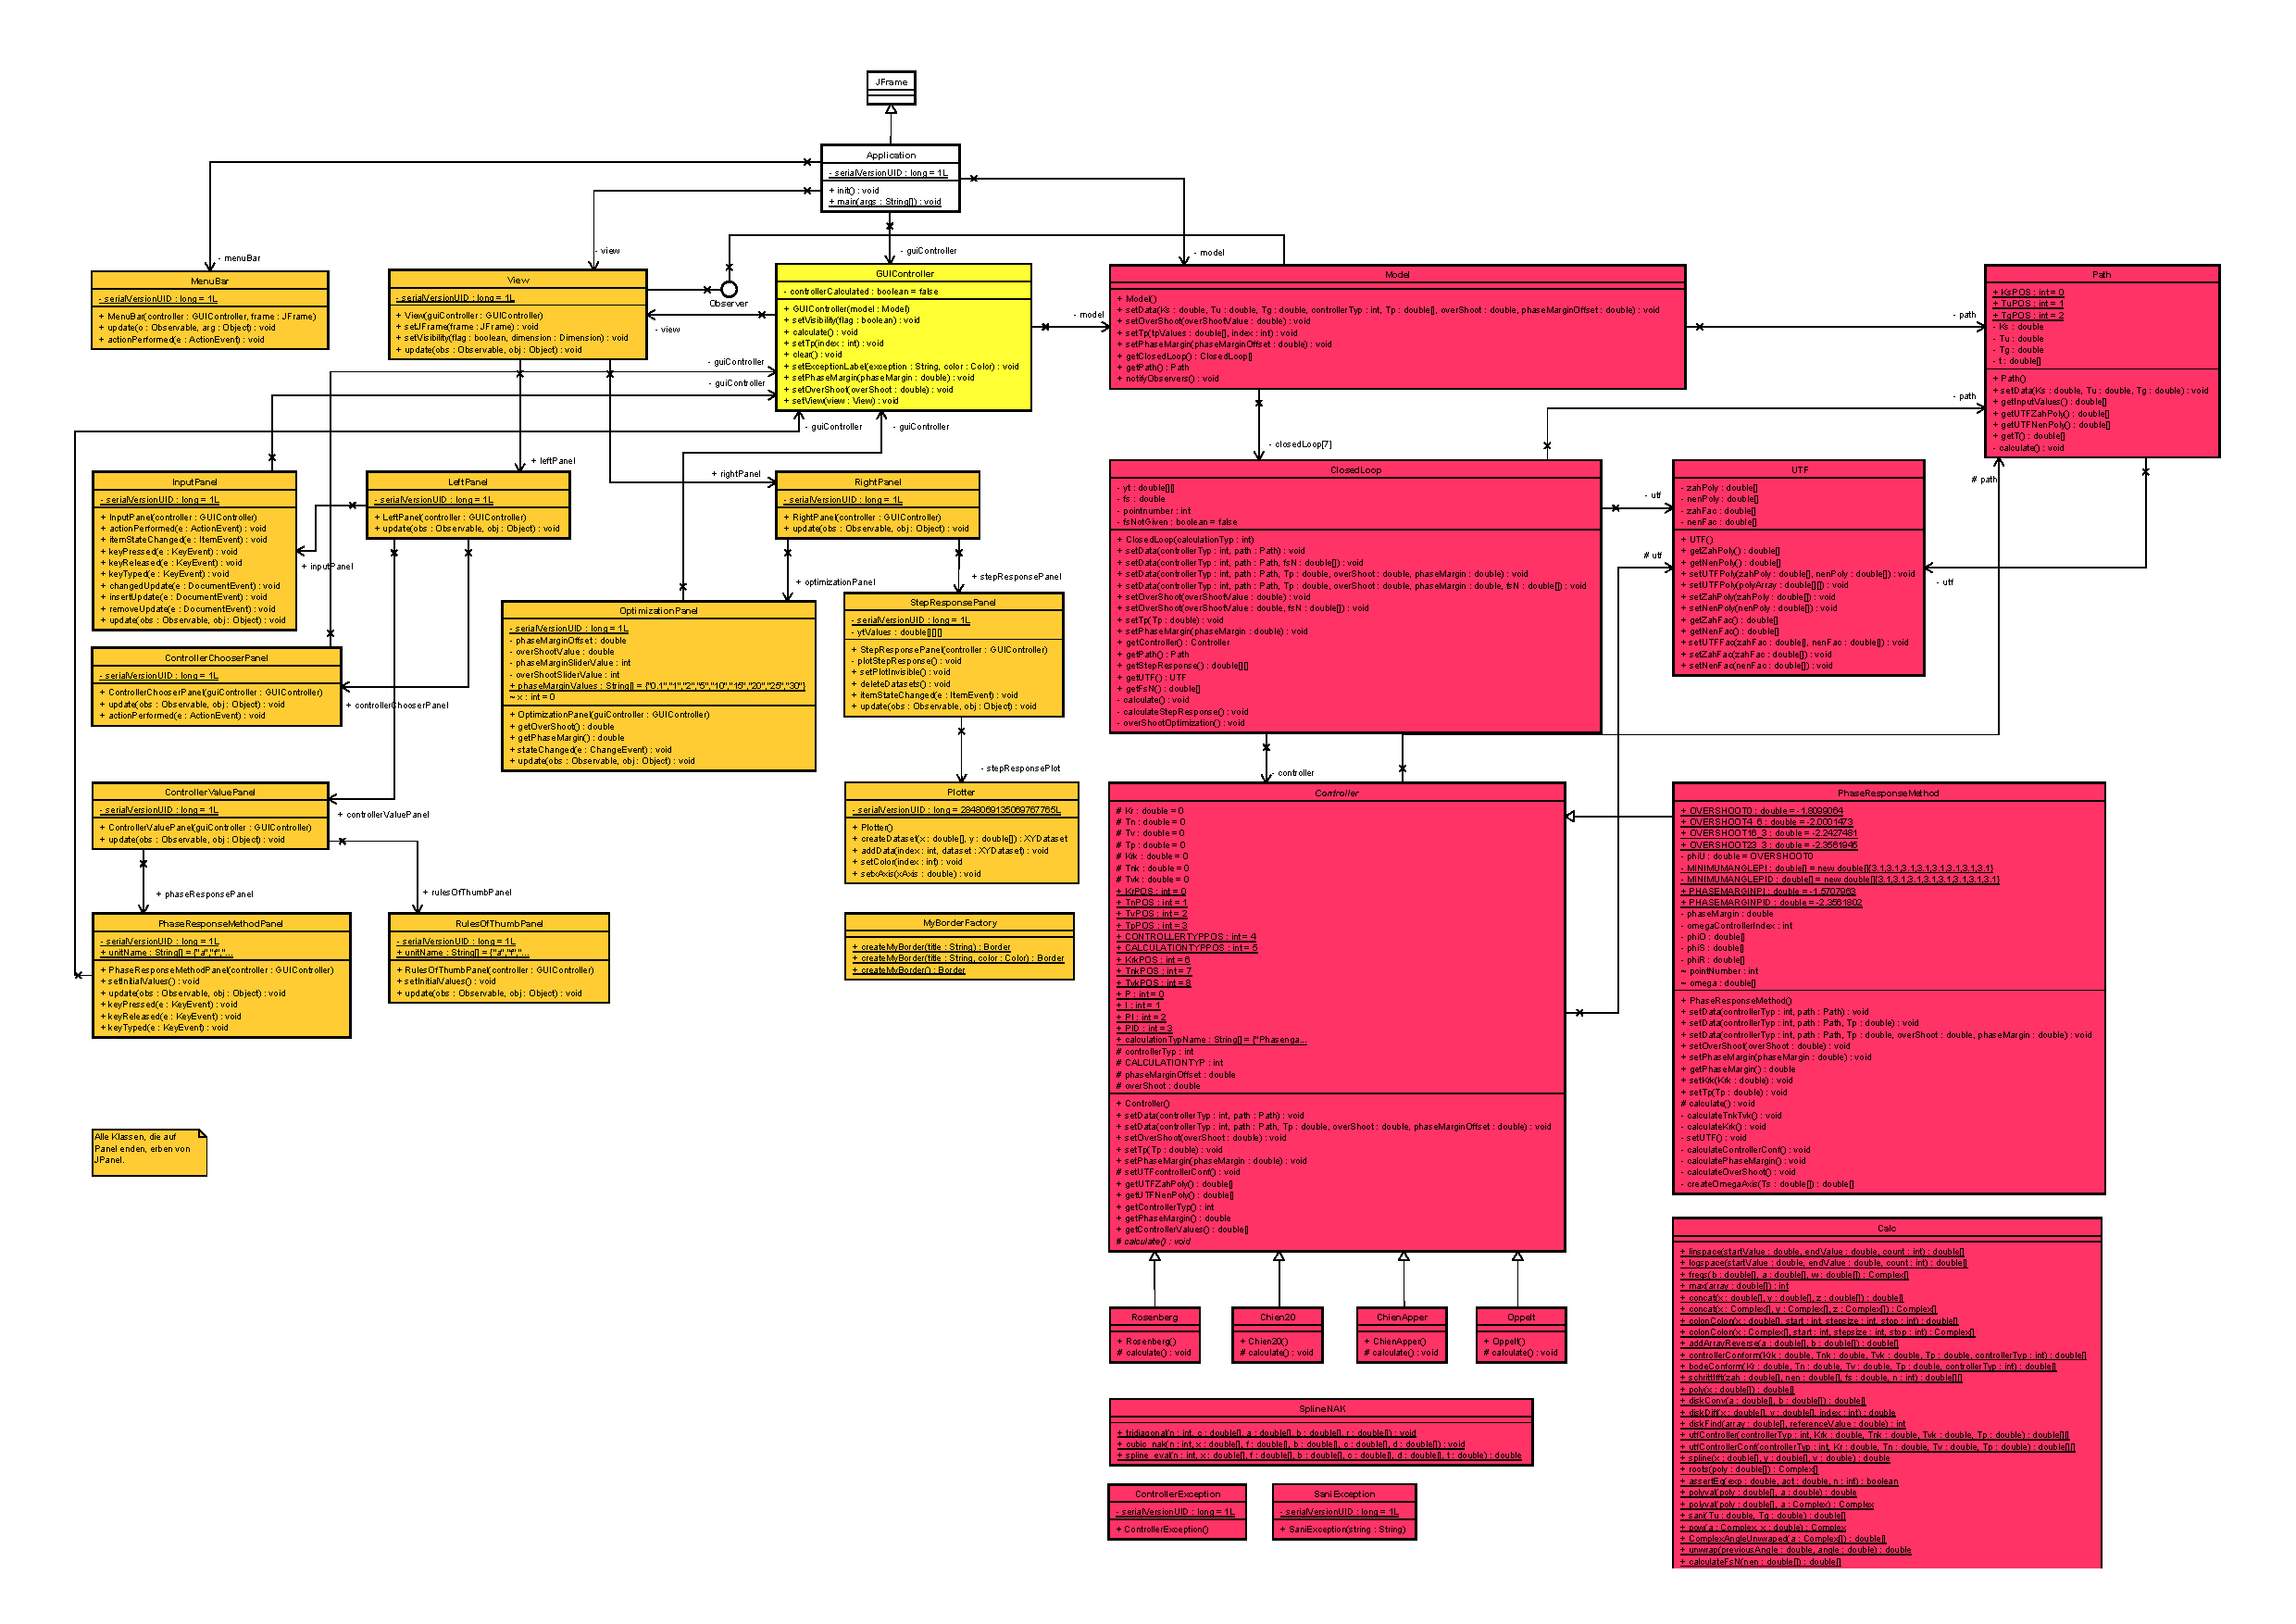
\includepdf[pages=1,scale=1]{images/klassendiagramm.pdf}

\setlength\paperheight{297mm}
\setlength\paperwidth{210mm}
\setlength\pdfpageheight{\paperheight}
\setlength\pdfpagewidth{\paperwidth}




% **************************************************************************** %
%\cleardoublepage
%\phantomsection
%\addcontentsline{toc}{section}{\listigurename}
%\listoffigures
% **************************************************************************** %


% **************************************************************************** %
\clearpage
\phantomsection
\addcontentsline{toc}{section}{\bibname}
\bibliography{bibliography/bibliography}{\bibliographystyle{bibliography/deIEEEtran.bst}}
% **************************************************************************** %

\end{document}
